\documentclass[]{article}

\usepackage{parskip}
\usepackage{microtype}
%\usepackage[T1]{fontenc}¡

\usepackage{graphicx}
%\usepackage{caption}
\graphicspath{{Fotos/}}

\usepackage{cancel}

\usepackage{amsmath}
\usepackage{amsfonts}
\usepackage{wasysym}

% ddphonism
% 
% (c) Celia Rubio Madrigal
%
%% This program can be redistributed and/or modified under the terms
%% of the LaTeX Project Public License Distributed from CTAN archives
%% in directory macros/latex/base/lppl.txt.
 
\NeedsTeXFormat{LaTeX2e}
\ProvidesPackage{ddphonism}
[2019/08/10 v0.2 Dodecaphonic diagrams: twelve-tone matrices, clock diagrams, etc.]

\RequirePackage{etoolbox}
\RequirePackage{xparse}
\RequirePackage{tikz}
\RequirePackage{xstring}
\RequirePackage{pgfkeys}


%%%%%%%%%%%%%%%%%%%%%%%%%%%%%%%%%%%%
% Matrices

\usetikzlibrary{matrix}

\ExplSyntaxOn
\DeclareExpandableDocumentCommand{\Evaluation}{m}{\int_eval:n {#1}}
\ExplSyntaxOff

\newcounter{Dsize}
\newcommand{\DsizeMake}[1]{%
	\setcounter{Dsize}{0}%
	\foreach \n in {#1}{%
		\stepcounter{Dsize}%
	}%
}

% Only with numbers.
\newcounter{Dfirst}
\newcommand{\DheadMake}[1]{%
	\setcounter{Dfirst}{-1}%
	\foreach \n in {#1}{%
		\ifnum\theDfirst=-1%
		\setcounter{Dfirst}{\n}%
		\fi%
	}%
}

% Only when DsizeMake is already done.
\newcounter{Dmod}
\newcommand{\Modulo}[1]{%
	\setcounter{Dmod}{#1}%
	\loop%
	\ifnum\theDmod>\Evaluation{\theDsize-1}%		
		\setcounter{Dmod}{\Evaluation{\theDmod-\theDsize}}%
		\repeat%
	\ifnum\theDmod<0%
		\setcounter{Dmod}{\Evaluation{\theDmod+\theDsize}}%
		\repeat%
	\theDmod%
}

\newif\ifdmatrixLines
\newif\ifdmatrixOutside
\newif\ifdmatrixInside
\newif\ifdmatrixV
\newif\ifdmatrixH
\newif\ifdmatrixTikz
\pgfkeys{
	/dmatrix/.is family
	, /dmatrix
	, default/.style = 
		{ lines = false
		, outside lines = false
		, inside lines = false
		, sep = 1
		, vsep = 1
		, hsep = 1
		, no tikz = false
		}
	, no tikz/.is if=dmatrixTikz
	, lines/.is if=dmatrixLines
	, outside lines/.is if=dmatrixOutside
	, inside lines/.is if=dmatrixInside
	, vlines/.is if=dmatrixV
	, hlines/.is if=dmatrixH
	, sep/.estore in=\dmatrixSep
	, vsep/.estore in=\dmatrixVsep
	, hsep/.estore in=\dmatrixHsep
}

\newcommand{\DLOH}{%
	\draw (0.05*\dmatrixSep*\dmatrixHsep,0) --%
	(\theDsize*\dmatrixSep*\dmatrixHsep+0.05*\dmatrixSep*\dmatrixHsep,0);%
	\draw (0.05*\dmatrixSep*\dmatrixHsep,-\theDsize*0.5*\dmatrixSep*\dmatrixVsep) -- %
	(\theDsize*\dmatrixSep*\dmatrixHsep+0.05*\dmatrixSep*\dmatrixHsep,-\theDsize*0.5*\dmatrixSep*\dmatrixVsep);%
}

\newcommand{\DLOV}{%
	\draw (0.05*\dmatrixSep*\dmatrixHsep,0) -- %
	(0.05*\dmatrixSep*\dmatrixHsep,-\theDsize*0.5*\dmatrixSep*\dmatrixVsep);%
	\draw (\theDsize*\dmatrixSep*\dmatrixHsep+0.05*\dmatrixSep*\dmatrixHsep,0) -- %
	(\theDsize*\dmatrixSep*\dmatrixHsep+0.05*\dmatrixSep*\dmatrixHsep,-\theDsize*0.5*\dmatrixSep*\dmatrixVsep);
}

\newcommand{\DLIH}{%
	\draw (0.05*\dmatrixSep*\dmatrixHsep,-\xD*0.5*\dmatrixSep*\dmatrixVsep) -- %
	(\theDsize*\dmatrixSep*\dmatrixHsep+0.05*\dmatrixSep*\dmatrixHsep,-\xD*0.5*\dmatrixSep*\dmatrixVsep);%
}

\newcommand{\DLIV}{%
	\draw (\xD*\dmatrixSep*\dmatrixHsep+0.05*\dmatrixSep*\dmatrixHsep,0) -- %
	(\xD*\dmatrixSep*\dmatrixHsep+0.05*\dmatrixSep*\dmatrixHsep,-\theDsize*0.5*\dmatrixSep*\dmatrixVsep);%
}

\newcommand{\dmatrix}[2][]{%
	\DsizeMake{#2}%
	\DheadMake{#2}%
	%
	\pgfkeys{/dmatrix, default, #1}%
	%
	\ifdmatrixTikz\else%
	\begin{tikzpicture}%
	\fi%
	\foreach [count=\nj] \j in {#2} {%
		\foreach [count=\ni] \i in {#2} {%
			\draw node at 
			( \ni*\dmatrixSep*\dmatrixHsep-0.5*\dmatrixSep*\dmatrixHsep
			, -\nj*\dmatrixSep*\dmatrixVsep/2+0.25*\dmatrixSep*\dmatrixVsep) {%
				\Modulo{\Evaluation{\i-\j+\theDfirst}}%
			};%
		}%
	}%
	\foreach \xD in {1,...,\Evaluation{\theDsize-1}} {%
		\ifdmatrixLines
		\DLOH\DLOV\DLIH\DLIV
		\fi
		\ifdmatrixOutside
		\DLOH\DLOV
		\fi
		\ifdmatrixInside
		\DLIH\DLIV
		\fi
		\ifdmatrixH
		\DLOH\DLIH
		\fi
		\ifdmatrixV
		\DLOV\DLIV
		\fi
	}%
%
\ifdmatrixTikz\else%
\end{tikzpicture}%
\fi%
}


%%%%%%%%%%%%%%%%%%%%%%%%%%%%%%%%%%%%
% Diagrams

\usetikzlibrary{shapes,arrows,decorations.markings,shapes.misc}

\tikzstyle ddiagramArrow=[decoration=
		{markings,mark=at position 0.25 with
			{\arrow[scale=1.25,>=triangle 45]{>}}},
	postaction={decorate}]

\tikzstyle{ddiagram}=[minimum height=0pt,inner sep=0pt,outer sep=0pt,scale=0.65]

\newif\ifddiagramTikz
\pgfkeys{
	/ddiagram/.is family
	, /ddiagram
	, default/.style = 
		{ name =\empty%
		, up =\empty%
		, no tikz = false
		}
	, no tikz/.is if=ddiagramTikz
	, name/.estore in=\ddiagramName
	, up/.estore in=\ddiagramUp
}

\newcounter{Dprev}
\newcommand{\Dvar}{}
\newcommand{\ddiagram}[2][]{%
	\DsizeMake{#2}%
	\DheadMake{#2}%
	%
	\pgfkeys{/ddiagram, default, #1}%
	%
	\ifdefequal{\ddiagramUp}{\empty}%
	{\renewcommand{\Dvar}{\theDfirst}}% if empty
	{\renewcommand{\Dvar}{\ddiagramUp}}% if not empty
	%
	\ifddiagramTikz\else%
	\begin{tikzpicture}[ddiagram,rotate=360*\Dvar/\theDsize]%
	\fi%
	\foreach \x in {0,...,\Evaluation{\theDsize-1}} {%
		\node at (90-360*\x/\theDsize:2) {\x};%
		\node (\x) at (90-360*\x/\theDsize:1.6) {};%
	};%
	%
	\setcounter{Dprev}{-1}%
	\foreach \x in {#2}{%
		\ifnum \theDprev=\theDfirst%
		\draw [style=ddiagramArrow] (\theDprev) -- (\x);%
		\else \ifnum \theDprev=-1%
		\else%
		\draw (\theDprev) -- (\x);%
		\fi\fi%
		\setcounter{Dprev}{\x}%
	};%
	\draw (\theDprev) -- (\theDfirst);%
	%
	\ifdefequal{\ddiagramName}{\empty}%
	{}% if empty
	{\node at (0,0) [circle,fill=white] {\ddiagramName};}% if not empty
	\ifddiagramTikz\else%
	\end{tikzpicture}%
	\fi%
}


%%%%%%%%%%%%%%%%%%%%%%%%%%%%%%%%%%%%
% Dihedral diagrams

\tikzstyle ddihedralArrow=[decoration=
		{markings,mark=at position 1 with {\arrow[scale=1.5,>=angle 60]{>}}},
	postaction={decorate}]

\tikzstyle{ddihedral}=[inner sep=0,minimum height=18pt]

\newif\ifddihedralTikz
\pgfkeys{
	/ddihedral/.is family, /ddihedral,
	default/.style = {t = 0, c = 0, s = 0, v = 0, no tikz=false},
	no tikz/.is if=ddihedralTikz,
	t/.estore in = \ddihedralT,
	c/.estore in = \ddihedralC,
	s/.estore in = \ddihedralS,
	v/.estore in = \ddihedralV,
}

\newif\ifdarrowsTikz
\pgfkeys{
	/darrows/.is family, /darrows,
	default/.style = {no tikz=false},
	no tikz/.is if=darrowsTikz,
}
\newcommand{\darrows}[2][]{%
	\DsizeMake{#2}%
	%
	\pgfkeys{/darrows, default, #1}%
	%
	\ifdarrowsTikz\else%
	\begin{tikzpicture}%
	\fi%
	\draw foreach \x in {0,...,\Evaluation{\theDsize-1}} {%
		(90-360*\x/\theDsize:2.5) node[circle] (\x) {}%
	};%
	\foreach \x [count=\y] in {#2} {%
		\draw [style=ddihedralArrow] (90-360*\Evaluation{\y-1}/\theDsize:1.25) -- (\x);%
	};%
	\ifdarrowsTikz\else%
	\end{tikzpicture}%
	\fi%
}

\newcommand\ddihedral[2][]{%
	\DsizeMake{#2}%
	%
	\pgfkeys{/ddihedral, default, #1}%
	%
	\ifddihedralTikz\else%
	\begin{tikzpicture}[ddihedral]%
	\fi%
	\draw foreach \x in {0,...,\Evaluation{\theDsize-1}} {%
		(\Evaluation{(90+\ddihedralT*360/\theDsize)+(2*\ddihedralS-1)*\x*360/\theDsize}:2.5)%
		node[very thin,circle,draw] (\x) {\x}%
	};%
	%
	\draw foreach \x in {0,...,\Evaluation{\theDsize-1}} {%
		(\Evaluation{(90-\ddihedralC*360/\theDsize)+(2*\ddihedralV-1)*\x*360/\theDsize}:1.25)%
		node[very thin,circle,draw] {\x}%
	};%
	%
	\darrows[no tikz]{#2}%
	%
	\node at (0,0) [very thin,draw,circle, fill=white] {%
		\ifnum\ddihedralV=0%
		\ifnum\ddihedralC=0%
		\ifnum\ddihedralS=0%
		\ifnum\ddihedralT=0%
		P%
		\fi\fi\fi%
		\else V\fi%
		\ifnum\ddihedralC=0%
		\else C$^{\ddihedralC}$\fi%
		\ifnum\ddihedralS=0%
		\else S\fi%
		\ifnum\ddihedralT=0%
		\else T$^{\ddihedralT}$\fi%
	};%
	\ifddihedralTikz\else%
	\end{tikzpicture}%
	\fi%
}


%%%%%%%%%%%%%%%%%%%%%%%%%%%%%%%%%%%%
% Rows

\pgfkeys{
	/drow/.is family, /drow,
	default/.style = {sep=\arraycolsep},
	sep/.estore in = \drowSep,
}

\long\def\addto#1#2{\expandafter\def\expandafter#1\expandafter{#1#2}}
\newcounter{myDDcntr}
\newlength{\Dvarr}
	
\newcommand{\drow}[2][]{%
	\DsizeMake{#2}%
	%
	\pgfkeys{/drow, default, #1}%
	\setlength{\Dvarr}{\arraycolsep}
	\setlength{\arraycolsep}{\drowSep}
	%
	\ifnum\theDsize=0%
	\ensuremath{\left(\right)}%
	\else\ifnum\theDsize=1%
	\ensuremath{%
		\left(\begin{array}{*{\theDsize}c}%
			0\\%
			#2\\%
		\end{array}\right)%
	}%
	\else%
	\def\TableDDdata{}%
	\setcounter{myDDcntr}{0}%
	\loop%
	\addto\TableDDdata{\themyDDcntr\stepcounter{myDDcntr} &}%
	\stepcounter{myDDcntr}%
	\ifnum\themyDDcntr<\Evaluation{\theDsize-1}%
	\repeat%
	\addto\TableDDdata{\themyDDcntr \\}%
	\setcounter{myDDcntr}{0}%
	%
	\ensuremath{%
		\left(\begin{array}{*{\theDsize}c}%
			\TableDDdata%
			\StrSubstitute{#2}{,}{&}\\%
		\end{array}\right)%
	}%
	\fi\fi%
	\setlength{\arraycolsep}{\Dvarr}
}


%%%%%%%%%%%%%%%%%%%%%%%%%%%%%%%%%%%%
% Chord diagram

\newcommand{\dchords}[2][]{
	\DsizeMake{#2}
	\begin{tikzpicture}[ddihedral]
	\foreach[count=\nx] \x in {#2} {
		\node (\x) at (90+360/\theDsize-\nx*360/\theDsize:2) {};
	}
	\foreach \x in {#2} {
		\ifnum\Evaluation{\x-\theDsize/2}<0
		\ifodd\theDsize
		\draw (\x) -- (\Evaluation{\x+\theDsize/2-1});
		\else
		\draw (\x) -- (\Evaluation{\x-\theDsize/2});
		\fi\fi
	}
	\foreach[count=\nx] \x in {#2} {
		\node[very thin,circle,draw,fill=white] (\x) at (90+360/\theDsize-\nx*360/\theDsize:2) {\x};
	}
	\end{tikzpicture}
}

\usetikzlibrary{
	knots,
	hobby,
	decorations.pathreplacing,
	shapes.geometric,
	calc
}

\endinput


%% End of file `ddphonism.sty'.

\usepackage{multicol}
%\usepackage{vwcol}

\usepackage{hyperref}
%\usepackage{qrcode}

%\usepackage{listingsutf8}
%\lstset{
%	inputencoding=utf8,
%	extendedchars=true,
%	literate=%
%	{á}{{\'a}}1
%	{é}{{\'e}}1
%	{í}{{\'i}}1
%	{ó}{{\'o}}1
%	{ú}{{\'u}}1
%	{Á}{{\'A}}1
%	{É}{{\'E}}1
%	{Í}{{\'I}}1
%	{Ó}{{\'O}}1
%	{Ú}{{\'U}}1
%	{ñ}{{\~n}}1
%	{Ñ}{{\~N}}1
%	{¿}{{>}}1
%	{¡}{{<}}1
%	{―}{{---}}1
%}
\usepackage{pdfpages}

\newcommand{\apendices}
{\part*{ANEXOS}%
	\addcontentsline{toc}{part}{ANEXOS}
	%	\setcounter{chapter}{0}%
	\setcounter{section}{0}%
	\setcounter{subsection}{0}%
	\setcounter{subsubsection}{0}%
	%	\renewcommand\thechapter{\Alph{chapter}}
	%	\renewcommand{\chaptername}{Anexo}
	\renewcommand\thesection{\Alph{section}}
	%	\renewcommand{\secname}{Anexo}
}


\begin{document}
	
	\section{Introducci�n hist�rica del dodecafonismo}\label{ch:historia}

En esta secci�n describiremos cu�l fue el ambiente hist�rico y filos�fico en el que se cultiv� el primer modelo de serialismo musical: el \textbf{dodecafonismo}. A trav�s de su historia analizaremos por qu� el serialismo no fue una decisi�n aleatoria ni espont�nea, sino que surgi� de una necesidad est�tica de aquel periodo.
%
Vamos a comenzar con una breve cr�nica de la disonancia, tras lo cual describiremos las fases por las que el creador del dodecafonismo, Arnold Schoenberg, tuvo que pasar antes de concebirlo. %La disonancia desempe�� un papel fundamental en la g�nesis del dodecafonismo, como veremos enseguida.

\subsection{La historia de la disonancia}
La disonancia siempre ha formado parte de la experiencia musical. Con la m�sica ha venido siempre emparejada la disonancia, mano a mano, como instrumento de contraste, confrontaci�n y ruptura, pero tambi�n como elemento constructivo del discurso musical.

En la Antigua Grecia, la armon�a musical se consideraba unida al resto del universo. La rotaci�n de los astros emit�a sonidos arm�nicos, y era la armon�a la que apaciguaba el alma. Pero �qu� era la armon�a sino la uni�n de consonancia y disonancia? Como dijo Arist�teles:
\begin{quote}
\emph{El alma es armon�a porque la armon�a es mezcla y s�ntesis de contrarios, y de contrarios precisamente est� compuesto el cuerpo.}\\
{\footnotesize (Tomado de \cite{mha} J. de Aixquivel, \textit{Memorias de Historia Antigua}, 1989.)}
\end{quote}

Es bien sabido que la Escuela de Pit�goras, con su estudio sobre proporciones entre notas, buscaba encontrar cu�les eran los intervalos m�s consonantes: eran aquellos cuyo ratio formaba una relaci�n sencilla. El intervalo de octava era consonante porque su ratio era de 2:1, y de igual manera ocurr�a con los intervalos de quinta (3:2) y cuarta (4:3), a los que Arist�xeno comenz� a llamar \textit{s�mph$\bar{o}$nos} ($\sigma\acute{\upsilon}\mu\varphi\omega\nu o\varsigma$) \cite{cons}. En cambio, a los intervalos no tan sencillos se los llamaba \textit{di�ph$\bar{o}$nos} ($\delta\iota\acute{\alpha}\varphi\omega\nu o\varsigma$), y fue entonces cuando se le dio nombre a la disonancia.

Ya en la Edad Media, la polifon�a fue forjando normas sobre su uso. La primera regla compositiva de la m�sica occidental \textemdash seg�n Knud Jeppesen~\cite{jeppesen}\textemdash~fue la \emph{regla franconiana}, que expresaba que las disonancias deb�an ocurrir en la parte d�bil del comp�s, mientras que las consonancias en la parte fuerte. Es as� como los compositores trenzaban consonancia y disonancia al tejer los hilos de la m�sica.

Poco a poco la disonancia pas� a ser usada como floritura mel�dica: en notas de paso, apoyaturas o retardos, entre otras. Esta funci�n mel�dica fue impregnando el contrapunto hasta llegar a ser pieza clave en la continuidad de las voces. Adquiri� entonces una nueva funci�n contrapunt�stica, �y qui�n no se ha deleitado al escuchar una disonancia \textit{bachiana}?

Pero la disonancia estaba a�n inscrita a la tonalidad reinante. No fue hasta la introducci�n de acordes extra�os que la disonancia pas� a ser el centro del inter�s musical, y fue \textit{in crescendo} apropi�ndose del foco de atenci�n hasta llegar a ser m�s valiosa a�n que la consonancia. Para ello hubo que esperar hasta el siglo XIX, que fue testigo de un asombroso desarrollo del sistema arm�nico que acab� por quebrantar todas las preconcepciones musicales anteriores.

Para m�s informaci�n sobre la disonancia y su fascinante historia, recomendamos al lector el texto de Felipe Aguirre~\cite{aguirre}.

\subsection{Wagner, Mahler y la emancipaci�n de la disonancia}
Aunque las posibilidades que promet�a la tonalidad parec�an inagotables, sus l�mites comenzaron a percibirse hacia finales del siglo XIX. En palabras de Arnold Schoenberg:
\begin{quote}
\emph{El o�do se fue familiarizando gradualmente con gran n�mero de disonancias, hasta que lleg� a perder el miedo a su efecto perturbador.}\\
{\footnotesize Mencionado en \cite{scho} \emph{Composition with twelve tones}, de \emph{Style and Idea}, 1950.}
\end{quote}

Esta �poca culmin� con los dramas musicales de Richard Wagner, en los que todos los elementos de la obra estaban detalladamente estudiados por el compositor. A este concepto lo llamaba \emph{Gesamtkunstwerk} (``obra de arte total") \textemdash mencionado en \cite{wagner} \emph{Oper und Drama}, 1851\textemdash, ya que se aseguraba personalmente de que en sus �peras las artes esc�nicas, musicales, po�ticas y visuales se combinaran entre s� a la perfecci�n.

\begin{figure}[h]
\begin{center}
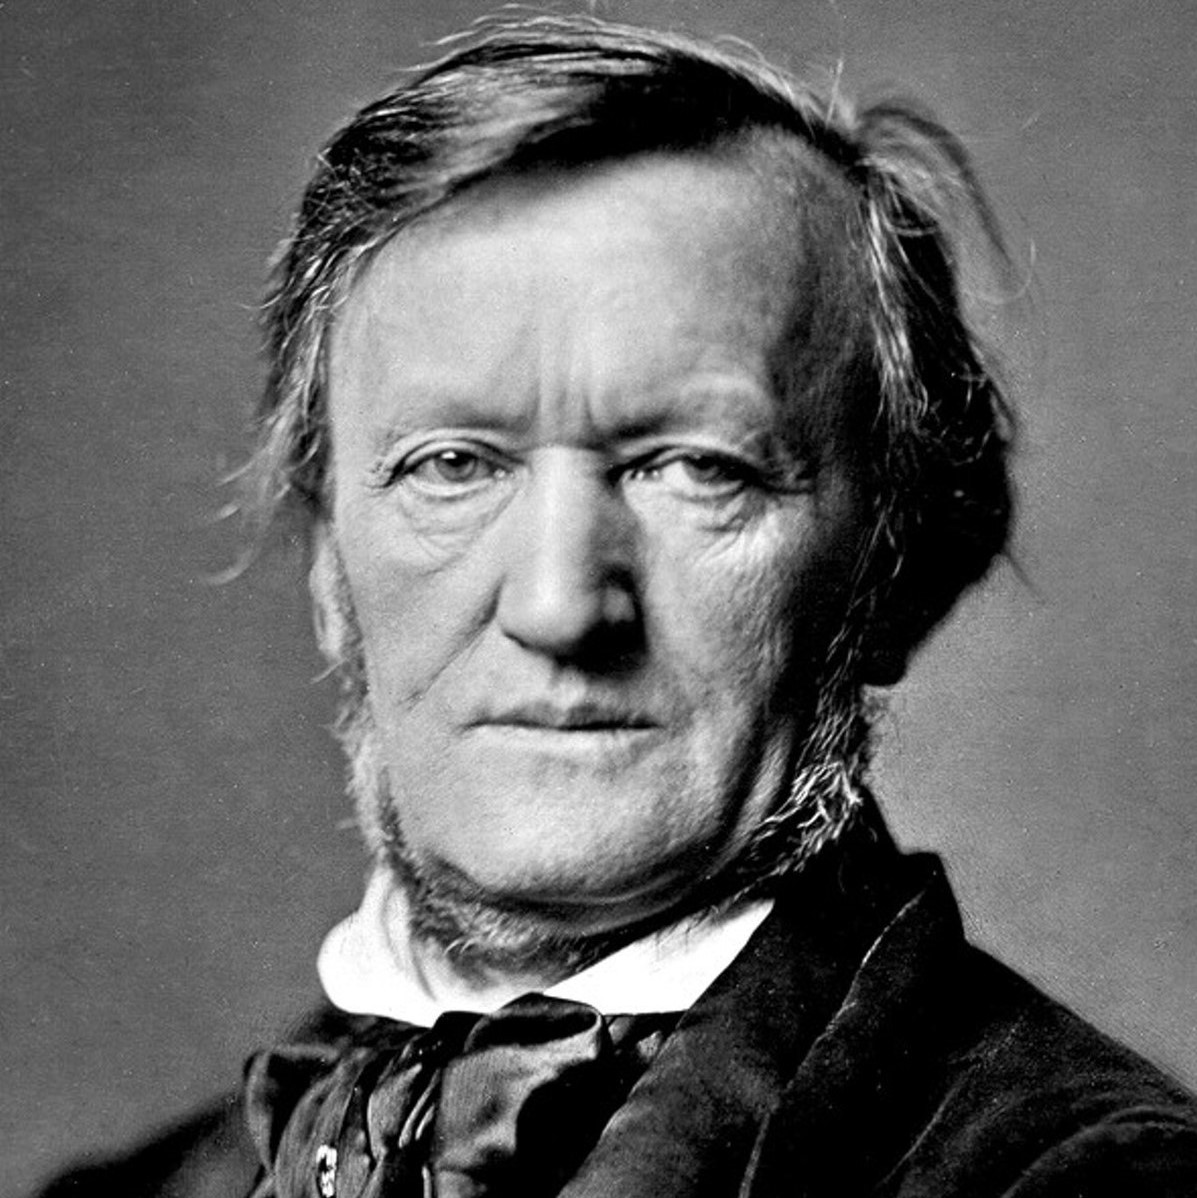
\includegraphics[width=5cm]{Richard_Wagner.jpg}\\
\caption{Richard Wagner (1813\textemdash1883); figura tomada de \href{https://www.nationalgeographic.com.es/historia/actualidad/richard-wagner-nacimiento-y-muerte_7014}{National Geographic}.}
\end{center}
\end{figure}

La idea del \emph{Gesamtkunstwerk} la desarroll� alrededor de 1850, y la plasm� en su totalidad en su ciclo de cuatro �peras \href{https://www.youtube.com/watch?v=1PBhlPeTJ_g}{\textit{Der Ring des Nibelungen}}, estrenado en 1876. Wagner control� y cre� cada aspecto de la tetralog�a, desde la m�sica hasta el libreto, el vestuario y la escenograf�a. Incluso mand� crear su propia sala de conciertos en Bayreuth, el \emph{Festspielhaus}, para que el escenario se adecuara a sus ideas sobre el pensamiento y la cultura musical; v�ase~\cite{kinney}.

As�, a ojos de compositores posteriores, se hab�an agotado todas las posibilidades de la m�sica tonal, y quiz�s ya hab�a comenzado el viraje hacia el predominio de la disonancia con su abundante uso del cromatismo, como en el famoso primer acorde del drama musical \href{https://www.youtube.com/watch?v=SF4zN-Okonc}{\textit{Tristan und Isolde}} (1865). Consta de las notas fa-si-$\mbox{re\#}$-$\mbox{sol\#}$, y sus intervalos desde el fa son una cuarta aumentada, una sexta aumentada y una novena aumentada.

Despu�s de Wagner, otros compositores tambi�n estuvieron a las puertas de emancipar la disonancia, de desatarla de las ataduras que impon�a la tonalidad. Por ejemplo, el gran compositor Gustav Mahler consegu�a reflejar en sus sinfon�as dos realidades paralelas: tanto la delicada fragilidad de la tradici�n anterior como la inminencia de su ruptura. El ejemplo m�s claro es el \href{https://www.youtube.com/watch?v=vHyV8noUXC0}{Adagio} de su D�cima Sinfon�a, que contiene una disonancia con once de las doce notas de la escala crom�tica. Y es que, sin lugar a dudas, la tonalidad ya preve�a que iba a ser reemplazada.

\begin{figure}[h]
\begin{center}
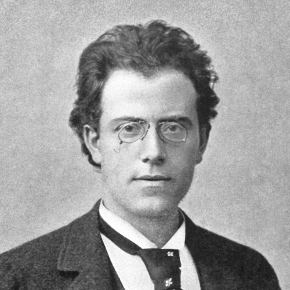
\includegraphics[width=5cm]{Gustav_Mahler.jpg}\\
\caption{Gustav Mahler (1860\textemdash1911); figura tomada de \href{http://www.planethugill.com/2018/09/mahler-distilled-iain-farrington-and.html}{Planet Hugill}.}
\end{center}
\end{figure}

Siguiendo la concepci�n del progreso como un camino ascendente, el paso siguiente para la composici�n musical deb�a consistir en deshacerse progresivamente de la tonalidad y desarrollar la ``{emancipaci�n de la disonancia}"  \textemdash mencionado tambi�n en \cite{scho} \emph{Composition with twelve tones}\textemdash. As�, en el marco expresionista del cambio de siglo, fue como Arnold Schoenberg ide� sus teor�as del pensamiento musical, y �stas dieron paso a la creaci�n de la atonalidad.

\subsection{Hacia el atonalismo de Schoenberg}
Fuertemente influido por Wagner y Mahler desde su adolescencia, Schoenberg comenz� componiendo al estilo posrom�ntico de su �poca, llevando el cromatismo y la orquestaci�n hasta el extremo. Sin embargo, y no espont�neamente, empez� a buscar en sus composiciones que cada sonido tuviera valor por s� mismo, un valor independiente de su funcionalidad tonal.

\begin{figure}[h]
\begin{center}
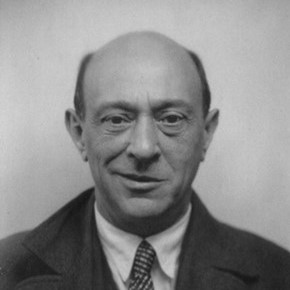
\includegraphics[width=5cm]{Arnold_Schoenberg.jpg}\\
\caption{Arnold Schoenberg (1874\textemdash1951); figura tomada de \href{http://es.nextews.com/59ce14c7/}{Nextews}.}
\end{center}
\end{figure}

Para �l, la m�sica no estaba intr�nsecamente dirigida a una t�nica. En las progresiones, lo importante era el paso de un acorde a otro, y no hacia d�nde se dirig�an estos. Adem�s, �l opinaba que se deb�an poder utilizar las notas de los modos eclesi�sticos libremente, por lo que consideraba las notas no diat�nicas tan v�lidas como las diat�nicas. Esto hac�a imposible distinguir unas de otras, y apenas se pod�a identificar la t�nica. De esta, y de otras muchas formas, Schoenberg consegu�a que la jerarqu�a tonal quedara desestabilizada~\cite{kinney}.

De esta �poca es su primera obra importante, \href{https://www.youtube.com/watch?v=vqODySSxYpc}{\emph{Verkl�rte Nacht}} ({\it Noche transfigurada}), Op. 4. Compuesto en 1899, este sexteto de cuerdas est� inspirado por el poema hom�nimo de Richard Dehmel. La m�sica, seg�n su autor, expresa el paseo de un hombre y una mujer en medio del abrazo de la naturaleza.  Aunque en la obra a�n prevalece la armon�a tradicional basada en acordes, Schoenberg sit�a al oyente en un terreno de indefinici�n tonal, no s�lo en el plano arm�nico sino tambi�n en el mel�dico. Adem�s, hace uso del acorde de novena invertido, inexistente hasta entonces y, por tanto, rechazado por la cr�tica~\cite{diaz}.

Tras pasar por la etapa tonal posrom�ntica, y debido a su convicci�n en la inexorabilidad de la evoluci�n de la m�sica hacia el cromatismo total, en 1908 Schoenberg se deslig� de la tonalidad completamente con el ciclo de canciones \href{https://www.youtube.com/watch?v=3iXsKhaZB2Q}{\emph{Das Buch der H�ngenden G�rten}}. 

A partir de entonces se dedic� a componer fragmentos muy breves cuya estructura era definida por motivos y no por la armon�a. Era esto lo que sol�a ocurrir en formas musicales anteriores como la forma sonata. A este periodo en sus composiciones se le llama atonalidad libre, aunque cabe destacar que Schoenberg rechazaba fervientemente este t�rmino:

\begin{quote}
\emph{La expresi�n ``m�sica atonal'' es de lo m�s desafortunada \textemdash es como llamar a volar ``el arte de no caer'' o nadar ``el arte de no ahogarse''.}\\
{\footnotesize Mencionado en \cite{hauer} A. Schoenberg, \emph{Hauer's Theories}, en \emph{Style and Idea}, 1923.}
\end{quote}

\noindent A este periodo pertenece tambi�n su famoso ciclo de canciones \href{https://www.youtube.com/watch?v=vQVkbKULKpI}{\emph{Pierrot Lunaire}}, Op. 21 (1912). Su nombre completo es \textit{Tres veces siete poemas de Pierrot Lunaire de Albert Giraud}, ya que est� dividida en 3 grupos de 7 canciones cada uno, cuyos textos son una selecci�n de 21 poemas del ciclo hom�nimo de Albert Giraud. 

Se encuentran en ella abundantes referencias al n�mero 7. Schoenberg hace un uso extensivo de motivos de 7 notas a lo largo de la obra, mientras que el conjunto musical que la interpreta, incluyendo al director, consta de 7 miembros. De hecho, a este conjunto de instrumentos \textemdash flauta, clarinete, viol�n, violonchelo, piano y voz\textemdash~se le ha dado el nombre de \textit{ensemble Pierrot} en su honor.  Otros n�meros importantes en la obra son el 3 y el 13. Cada poema consta de 13 l�neas, mientras que la primera l�nea de cada poema aparece 3 veces: en las l�neas 1, 7 y 13.

En esta obra no s�lo hay una ausencia total de relaciones tonales, sino que el tratamiento vocal evita tambi�n cualquier relaci�n est�tica con las t�cnicas tradicionales: es un \emph{Sprechgesang}, un canto hablado. De hecho, Schoenberg se refiere a estas piezas no como canciones, sino como melodramas. V�ase~\cite{diaz} para m�s informaci�n.

\subsection{El surgimiento del sistema dodecaf�nico}
Schoenberg no estaba a�n satisfecho con su t�cnica compositiva, ya que admiraba las obras extensas de los m�sicos rom�nticos y pensaba que su atonalidad no pod�a sostener una obra de gran envergadura. Es decir, necesitaba un hilo conductor mejor que los motivos para poder componer obras atonales m�s largas.

Por aquella �poca sufri� crisis en varios aspectos de su vida. En lo personal, su mujer Matilde Zemlinsky acababa de abandonarlo por otro hombre, aunque posteriormente volver�a junto al compositor. Y en lo profesional, sus obras no eran del gusto del p�blico, por lo que no contaba con suficiente dinero para mantener a su familia. Todas estas circunstancias, unidas al desarrollo de la Primera Guerra Mundial, no le permitieron componer apenas entre 1914 y 1923.

Tras el final de la guerra, en 1919, Schoenberg fund� la Sociedad para Interpretaciones Musicales Privadas junto a sus disc�pulos y amigos Alban Berg y Anton Webern. Schoenberg, Berg y Webern se autodenominaron la Segunda Escuela de Viena en honor al grupo de compositores del siglo XVIII Haydn, Mozart y Beethoven, quienes formaban la Primera Escuela de Viena.

En la Sociedad para Interpretaciones Musicales Privadas se presentaban m�sicas contempor�neas en circunstancias que favorecieran su adecuada apreciaci�n. As� se evitaba que dichas obras, al no ser entendidas por el p�blico, fueran inmediatamente rechazadas. Las obras de compositores como Mahler, Debussy, Bart�k, Ravel, Strauss y Stravinsky fueron incluidas en los programas de conciertos organizados por la Sociedad.

En este contexto Schoenberg pudo reflexionar sobre sus t�cnicas compositivas, y al fin public� en 1923 su ensayo \emph{M�todo de composici�n con doce sonidos}~\cite{scho}, donde se describ�an por primera vez los axiomas del dodecafonismo. Estos axiomas constitu�an la soluci�n al problema de la atonalidad libre que tanto le hab�a estado atormentando durante una d�cada.

Su primera obra �ntegramente dodecaf�nica, publicada tambi�n en 1923, es la Suite para piano Op. 25, que podr�n ver a continuaci�n. Es la pieza m�s temprana en la que Schoenberg usa series dodecaf�nicas en cada uno de los movimientos. En dos obras anteriores a ella usa series dodecaf�nicas, pero en movimientos aislados: la Op. 23, \href{https://www.youtube.com/watch?v=7A9HSlgDlQE}{\emph{5 St\"ucke}} (1920\textemdash23), en el movimiento de Waltz final; y su \href{https://www.youtube.com/watch?v=fzAFalLbXxg}{Serenata}, Op. 24, en su Soneto central.

Las series utilizadas en la Suite Op. 25 servir�n de ejemplo en este texto, y su tercer movimiento, \href{https://www.youtube.com/watch?v=scwNtGdop6w}{Musette}, ser� estudiado y analizado en el apartado \ref{musette} con el fin de entender una obra dodecaf�nica en toda su extensi�n. A continuaci�n el lector podr� escuchar la Suite para piano Op. 25:

\xxx{Incluir v�deo}%
	\chapter[EL SISTEMA DODECAFÓNICO DE SCHOENBERG]{EL SISTEMA DODECAFÓ- NICO DE SCHOENBERG}
	\section{Los postulados del dodecafonismo}
		El dodecafonismo es un sistema compositivo que predetermina la melodía y la armonía a partir de una ordenación de las doce notas de la escala cromática, que se llama \textit{serie}. Ésta y algunas de sus transformaciones son los ladrillos con los que se construyen las alturas de las notas; son el único material que se puede utilizar. \cite{delgado}
		
		El resto de elementos de la pieza, como el número de instrumentos, el ritmo, el carácter, la textura o las dinámicas, se dejan a discreción del compositor. No serializar todos los conjuntos será la principal crítica al dodecafonismo por parte de los compositores serialistas que sucedieron a su creador, Arnold Schoenberg. Para los serialistas integrales, como Pierre Boulez, aquello restaba cohesión al modelo compositivo; para los dodecafonistas, aportaba libertad. \cite{boulez}
		
		Precisamente la predeterminación dodecafónica, aunque parece limitante, permite realizaciones musicales y estilos de composición muy diferentes: Schoenberg daba un tratamiento tradicional a sus obras, ya que aún admiraba las formas clásicas; Alban Berg iba más allá al utilizar series que recordaban a las tríadas tonales; y, en cambio, Anton Webern evitaba radicalmente cualquier asociación con la tradición. \cite{delgado}
		
		Schoenberg definió su sistema musical a partir de cuatro postulados que, en realidad, se basan en principios matemáticos \cite{dominguez}:
		
		\emph{1. La serie \emph{[sobre la que se construye la obra dodecafónica]} consta de las doce notas de la escala cromática dispuestas en un orden lineal específico.}
		
		\emph{2. Ninguna nota aparece más de una vez en la serie.}
		
		Los dos primeros postulados expresan que una obra dodecafónica fundamenta su estructura sobre una permutación de la escala de doce semitonos. Dicha permutación $\sigma$ es una biyección del conjunto numerado de las doce notas \{Do = 0, Do\# = 1, Re = 2, Re\# = 3, Mi = 4, Fa = 5, F\# = 6, Sol = 7, Sol\# = 8, La = 9, La\# = 10, Si = 11\} consigo mismo, y se representa de esta forma:
		
		\full{
			\drow{
				\sigma(0),\sigma(1),\sigma(2),\sigma(3),\sigma(4),\sigma(5),\sigma(6),\sigma(7),\sigma(8),\sigma(9),\sigma(10),\sigma(11)
			}
		}
	
		La permutación $\sigma(m)$, con $m\in \mathbb{Z} / (12)$\footnote{$\mathbb{Z} / (12)=\{0,\ 1,\ 2,\ 3,\ 4,\ 5,\ 6,\ 7,\ 8,\ 9,\ 10,\ 11\}$}, pertenece al grupo simétrico de orden 12: $\sigma\in$ S$_{12}$. Por ejemplo, en la Suite para piano Op. 25 Schoenberg utiliza como serie original en todos los movimientos de la obra la siguiente permutación $\sigma$:
		
		\[\sigma=\drow{4,5,7,1,6,3,8,2,11,0,9,10}\]	
		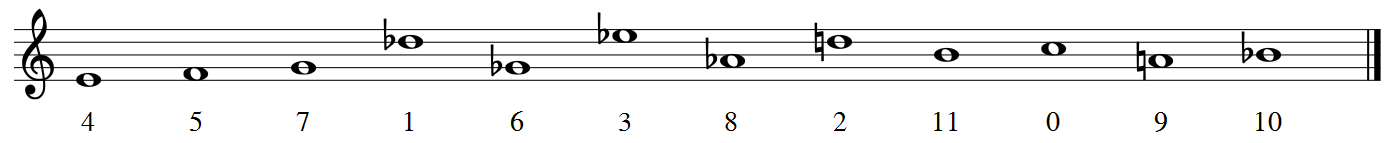
\includegraphics[width=\textwidth]{1.png}
		
		\emph{3. La serie será expuesta en cualquiera de sus aspectos lineales: original, inversión, retrogradación de la original y retrogradación de la inversión.}
		 
		\emph{4. La serie puede usarse en sus cuatro aspectos desde cualquier nota de la escala.}
		
		Los dos últimos postulados amplían los recursos compositivos al admitir la transformación de la serie original mediante \emph{inversión}, \emph{retrogradación}, \emph{inversión retrógrada} y \emph{transposición}\footnote{No confundir con un 2-ciclo. Una transposición musical se corresponde con una traslación matemática.}. El compositor puede utilizar cualquiera de las transformaciones de una serie al componer su obra dodecafónica. El conjunto de series que puede utilizar, que viene dado por la serie original y todas sus posibles transformaciones, se conoce como \emph{espectro serial}. \cite{dominguez}
		
	\section{Las transformaciones de una serie}
		\label{transPsi}
		Transformar una serie es matemáticamente equivalente a aplicar una función sobre la serie, y que asocie esa permutación a la permutación transformada. Por tanto, cualquier función transformativa $\Psi$ se aplica sobre el conjunto de las permutaciones, S$_{12}$.
		
	\subsection{Transposiciones}
		La \emph{transposición}, mencionada en el cuarto postulado, consiste en subir o bajar la serie original un número determinado de semitonos. Por tanto, no se modifican los intervalos entre las notas, sino solamente la altura a la que está la serie. Ya que consideraremos todas las octavas equivalentes, debemos trabajar módulo 12. 
		
		La serie transportada k semitonos (con k constante), T$^\text{k}\left(\sigma\right)$, se construye sumando k a $\sigma$ (mod. 12):
		\[\text{T}^\text{k}\left(\sigma\left(m\right)\right)=\sigma\left(m\right)+\text{k}\]		
		\full{$
		\text{T}^\text{k}=
		\left(\begin{matrix}
			0&1&2&&9&10&11\\
			\sigma\left(0\right)+\text{k}&\sigma\left(1\right)+\text{k}&\sigma\left(2\right)+\text{k}&
			\cdots&
			\sigma\left(9\right)+\text{k}&\sigma\left(10\right)+\text{k}&\sigma\left(11\right)+\text{k}\\
		\end{matrix}\right)
		$}
		
		A su vez, T$^\text{k}$ se forma al componer k transposiciones de 1 semitono: $\text{T}^\text{k}=\text{T}^1\circ\text{T}^1\circ\ldots\circ\text{T}^1$, k veces. Debido a que k es en realidad el exponente en la potencia de T, se coloca este número como superíndice.
		
		Históricamente, la notación $\Psi_\text{k}$, $\Psi^\text{k}$ o $\Psi(\text{k})$ se ha usado en sustitución de la composición de la transposición T$^\text{k}$ y otra función $\Psi$, en el respectivo orden: $\Psi^\text{k}=\Psi \circ \text{T}^\text{k} = \Psi(\text{T}^\text{k})$. Sin embargo, esta notación es especialmente ambigua y confusa, sobre todo al trabajar con funciones no conmutativas. Por ello, es preferible ceñirse a la notación estrictamente matemática; es decir, a la composición de funciones, aun omitiendo $\circ$: \cancel{$\Psi_\text{k}$}, \cancel{$\Psi^\text{k}$}, \cancel{$\Psi(\text{k})$} $\rightarrow \Psi\text{T}^\text{k}$
		
		Una posible serie transportada sobre la permutación $\sigma$ de la Suite para piano Op. 25, con k $= 6$, es la siguiente serie T$^6$:
		\[\text{T}^6=\drow{10,11,1,7,0,9,2,8,5,6,3,4}\]	
		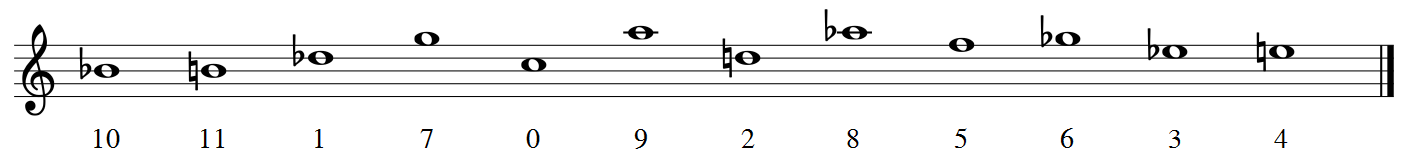
\includegraphics[width=\textwidth]{2.png}
		
	\subsection{Retrogradación}
		La \emph{retrogradación} consiste en leer la serie original desde la nota final hacia atrás, es decir, aplicar a la serie una simetría especular. De este modo, la primera nota irá al último puesto, la segunda al penúltimo, y así sucesivamente.
		
		La serie retrógrada se construye de esta forma:
		\[\text{R}\left(\sigma\left(m\right)\right)=\sigma\left(-1-m\right)\]
		\full{$\text{R}=\drow{\sigma(11),\sigma(10),\sigma(9),\sigma(8),\sigma(7),\sigma(6),\sigma(5),\sigma(4),\sigma(3),\sigma(2),\sigma(1),\sigma(0)}$}
			
		La serie retrógrada sobre la permutación $\sigma$ de la Suite Op. 25 es la siguiente serie R:	
		\[\text{R}=\drow{10,9,0,11,2,8,3,6,1,7,5,4}\]		
		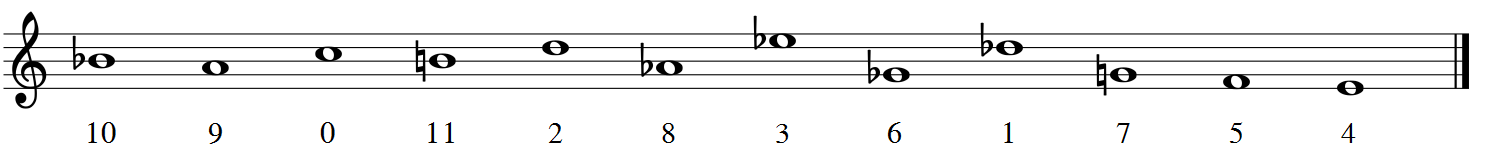
\includegraphics[width=\textwidth]{3.png}
		
	\subsection{Inversión}
		La \emph{inversión} consiste en cambiar la dirección --de ascendente a descendente, y viceversa-- de los intervalos entre cada nota de la serie. Si el primer intervalo en la serie original $\sigma$ es de $+k$, el primer intervalo en la serie invertida I será de $-k$ (mod. 12), por lo que debemos cambiar el signo de $\sigma$ para construir I. Además, queremos que la primera nota de ambas series, I(0) y $\sigma$(0), coincidan, así que debemos transportar la serie ($-\sigma$) un número $\lambda$ de semitonos para que esta condición se cumpla:
		\begin{align*}
		\text{I}(0)=-\sigma\left(0\right)+\lambda&=\sigma\left(0\right)\\
		\implies \lambda&=2\sigma(0)
		\end{align*}
		Por tanto, la serie invertida se construye de esta forma:
		\[\text{I}\left(\sigma\left(m\right)\right)=-\sigma\left(m\right)+2\sigma\left(0\right)\]
		\full{$
		\text{I}=\left(\begin{matrix}0&1&2&&10&11\\\sigma(0)&-\sigma(1)+2\sigma(0)&-\sigma(2)+2\sigma(0)&\ldots&-\sigma(10)+2\sigma(0)&-\sigma(11)+2\sigma(0)\\\end{matrix}\right)$}
		
		La serie invertida sobre la permutación $\sigma$ de la Suite Op. 25 es la siguiente serie I:
		\[\text{I}=\drow{4,3,1,7,2,5,0,6,9,8,11,10}\]		
		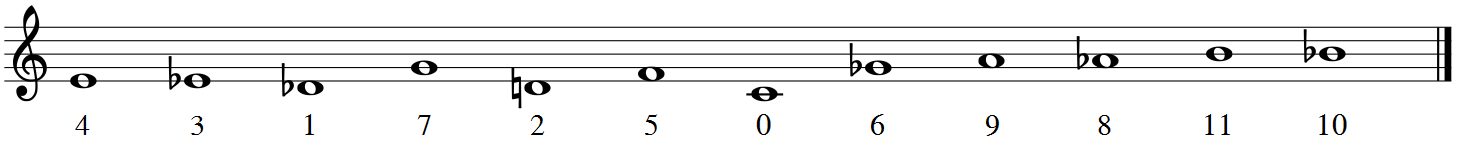
\includegraphics[width=\textwidth]{4.png}
				
		En total, obtendremos 48 series -- aunque no obligatoriamente distintas entre sí -- pertenecientes a un solo espectro serial. Hay 12 series originales sobre cada una de las doce notas, 12 series retrógradas, 12 invertidas y 12 series sobre las que se aplica tanto la retrogradación como la inversión. A continuación se muestra la sintaxis simple junto a la matemática:
		
		\begin{multicols}{2}
			\underline{Sintaxis simple}
			
			T$_0$, T$_1$, T$_2$\ldots
			
			R$_0$, R$_1$, R$_2$\ldots
			
			I$_0$, I$_1$, I$_2$\ldots
			
			IR$_0$, IR$_1$, IR$_2$\ldots
			
			\underline{Sintaxis matemática}
			
			T$^0$, T$^1$, T$^2$\ldots
			
			R, RT$^1$, RT$^2$\ldots
			
			I, IT$^1$, IT$^2$\ldots
			
			IR, IRT$^1$, IRT$^2$\ldots
		\end{multicols}
	
	\section{Matrices dodecafónicas}
		
		Dada una serie, su matriz dodecafónica es una representación visual de su espectro serial; es decir, del conjunto de series derivadas de esa serie. El espectro serial es todo el material compositivo sonoro del que se dispone para la composición de una obra dodecafónica. Al poder ordenar y disponer la información en una tabla, el compositor puede acceder a toda ella al mismo tiempo sin tener que calcular cada serie individualmente.		
		
		La matriz se lee en la dirección en la que aparece el nombre de la serie. Las series T se leen de izquierda a derecha, mientras que las series R de derecha a izquierda. Las series I se leen de arriba a abajo y las IR/RI de abajo a arriba.
		
		He creado un programa que devuelve en formato \LaTeX{} la matriz correspondiente a cualquier serie dodecafónica que se introduzca en teclado, además de producir la nomenclatura simple para cada serie. El código, escrito en C++, está incluido en el Anexo \ref{app:matrices}, página \pageref{app:matrices}.
		
		A continuación, se incluye la matriz dodecafónica de la serie P de la Suite Op. 25 de Schoenberg. Mientras que la mayoría de tablas tienen dos filas inferiores, que se corresponden con las distintas nomenclaturas de RI e IR para una misma serie – ya que normalmente no conmutan –, en la matriz de la serie P sí coinciden, como se mencionará en el apartado \ref{conmut}.
		
		\full{$\begin{array}{l|cccccccccccc|r}
		&\text{I}_{0}&\text{I}_{1}&\text{I}_{3}&\text{I}_{9}&\text{I}_{2}&\text{I}_{11}&\text{I}_{4}&\text{I}_{10}&\text{I}_{7}&\text{I}_{8}&\text{I}_{5}&\text{I}_{6}&\\
		\hline
		\text{T}_{0}&4&5&7&1&6&3&8&2&11&0&9&10&\text{R}_{0}\\
		\text{T}_{11}&3&4&6&0&5&2&7&1&10&11&8&9&\text{R}_{11}\\
		\text{T}_{9}&1&2&4&10&3&0&5&11&8&9&6&7&\text{R}_{9}\\
		\text{T}_{3}&7&8&10&4&9&6&11&5&2&3&0&1&\text{R}_{3}\\
		\text{T}_{10}&2&3&5&11&4&1&6&0&9&10&7&8&\text{R}_{10}\\
		\text{T}_{1}&5&6&8&2&7&4&9&3&0&1&10&11&\text{R}_{1}\\
		\text{T}_{8}&0&1&3&9&2&11&4&10&7&8&5&6&\text{R}_{8}\\
		\text{T}_{2}&6&7&9&3&8&5&10&4&1&2&11&0&\text{R}_{2}\\
		\text{T}_{5}&9&10&0&6&11&8&1&7&4&5&2&3&\text{R}_{5}\\
		\text{T}_{4}&8&9&11&5&10&7&0&6&3&4&1&2&\text{R}_{4}\\
		\text{T}_{7}&11&0&2&8&1&10&3&9&6&7&4&5&\text{R}_{7}\\
		\text{T}_{6}&10&11&1&7&0&9&2&8&5&6&3&4&\text{R}_{6}\\
		\hline
		&\text{IR}_{0}&\text{IR}_{1}&\text{IR}_{3}&\text{IR}_{9}&\text{IR}_{2}&\text{IR}_{11}&\text{IR}_{4}&\text{IR}_{10}&\text{IR}_{7}&\text{IR}_{8}&\text{IR}_{5}&\text{IR}_{6}&\\
		\hline
		&\text{RI}_{0}&\text{RI}_{1}&\text{RI}_{3}&\text{RI}_{9}&\text{RI}_{2}&\text{RI}_{11}&\text{RI}_{4}&\text{RI}_{10}&\text{RI}_{7}&\text{RI}_{8}&\text{RI}_{5}&\text{RI}_{6}&
		\end{array}$}
	
		Por otro lado, he escrito otro programa en el propio lenguaje \LaTeX{} que crea esta misma tabla con el comando \verb|\dmatrix|, y tiene cualquier serie como argumento: \verb|\dmatrix{4,5,7,1,6,3,8,2,11,0,9,10}|. El código se encuentra en el Anexo \ref{app:latex}, página \pageref{app:latex1}. La tabla aparece sin el orlado de nomenclaturas:
		\dmatrix{4,5,7,1,6,3,8,2,11,0,9,10}
	
		
		\bigbreak
		
		También he creado una página interactiva que genera matrices de cualquier serie para cualquier longitud serial, además de generar series aleatorias. Permite escoger entre dos numeraciones y dos nomenclaturas. Está escrita en Elm y el código puede encontrarse en \url{https://gitlab.com/dodecafonismo/matrices}.
		
		\begin{wrapfigure}{l}{0.2\textwidth}
			\vspace{-\bigskipamount}
			\qrcode{https://matrices.netlify.com/}
		\end{wrapfigure} En el código QR está el enlace de la aplicación web. Sus instrucciones de uso se encuentran al final de la página. El enlace es \url{https://matrices.netlify.com/}.
		
	\section{An�lisis de una obra dodecaf�nica: el opus 25}\label{ch:suite}
	\subsection{Series de la Suite op. 25}
		Lo primero que har� un compositor dodecaf�nico antes de empezar a componer ser� escoger su serie original. Su elecci�n nunca es una simple cuesti�n de azar; al contrario, ya que las singularidades de la serie dar�n un car�cter especial a toda la obra. Por ejemplo, el compositor puede escoger una serie con simetr�as, y as� tendr� series repetidas entre su espectro serial. Tambi�n puede tener simetr�as internas solo en un fragmento de tres o cuatro notas, y de este modo podr� el compositor oscilar entre varias series del espectro que se parezcan entre s�. Para un estudio m�s completo de las relaciones de similitud entre series se recomienda \emph{On the Similarity of Twelve-Tone Rows}, de Tuukka Ilom�ki \cite{ilomaki}.
		
		En la Suite para Piano Op. 25, Schoenberg escoge su serie $\sigma$ para resaltar el intervalo de tritono (6 semitonos). A continuaci�n se observan en negrita los intervalos entre las notas de esta serie, en unidad de semitono:
		
		\[\left(\begin{array}{*{24}c}
		0&&1&&2&&3&&4&&5&&6&&7&&8&&9&&10&&11&\\
		4&\mathbf{1}&5&\mathbf{2}&7&\mathbf{6}&1&\mathbf{5}&6&\mathbf{9}&3&\mathbf{5}&8&\mathbf{6}&2&\mathbf{9}&11&\mathbf{1}&0&\mathbf{9}&9&\mathbf{1}&10&\mathbf{6}\end{array}\right)\]
				
		Presenta repeticiones triples de los intervalos de tritono (6), de sexta mayor (9) y de segunda menor o semitono (1): los intervalos m�s disonantes; una repetici�n doble de cuarta justa (5), y un intervalo de segunda mayor (2); adem�s de una consecuci�n de intervalos repetida: 9--1--9--1. Como se forma el intervalo de tritono al enlazar la serie original con una serie que empiece por la misma nota, se tiene en cuenta el intervalo de tritono (6) al final. En el dodecafonismo se evitan deliberadamente los intervalos de tercera mayor (4), ya que estos son la base de la eludida armon�a tonal. \label{serie25}
		
		El intervalo de tritono tiene la particularidad de no modificarse en la inversi�n y transportaci�n k = 6, por lo que estos intervalos aparecen en los lugares originales, mientras que en los procedimientos de retrogradaci�n y retrogradaci�n inversa ocupan sus lugares en retr�grado. En particular, Schoenberg utiliza entre los seis movimientos de la Suite solamente las ocho series de todo el espectro serial que cumplen estos requisitos: $T^0$, $T^6$, $I$, $IT^6$, $R$, $RT^6$, $RI$ y $RIT^6$, que podemos observar a continuaci�n:
		
		\chapter{Series de la Suite Op. 25}
	\label{app:series}
	
	\newpage
	$$\text{T}^0=\left(\begin{matrix}0&1&2&3&4&5&6&7&8&9&10&11\\4&5&7&1&6&3&8&2&11&0&9&10\\\end{matrix}\right)$$
	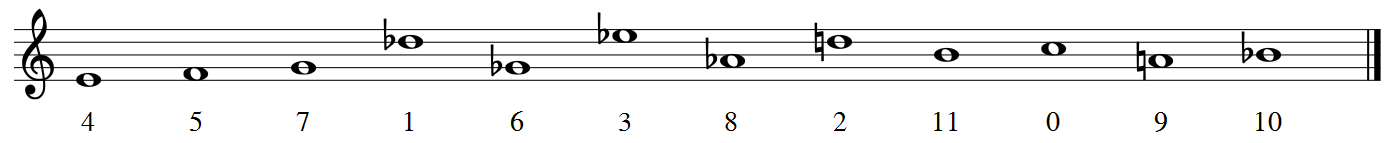
\includegraphics[width=\textwidth]{1.png}
	\bigskip\bigskip
	$$\text{T}^6=\left(\begin{matrix}0&1&2&3&4&5&6&7&8&9&10&11\\10&11&1&7&0&9&2&8&5&6&3&4\\\end{matrix}\right)$$
	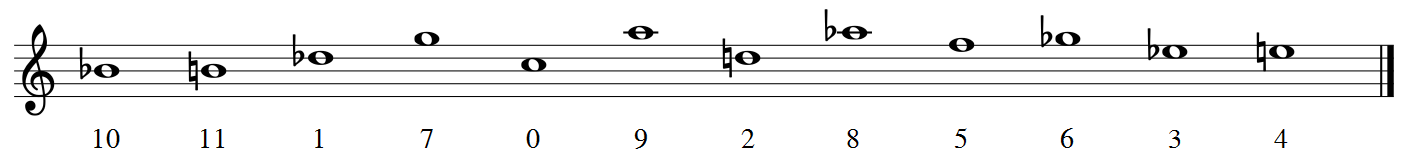
\includegraphics[width=\textwidth]{2.png}
	\bigskip\bigskip
	$$\text{IT}^0=\left(\begin{matrix}0&1&2&3&4&5&6&7&8&9&10&11\\4&3&1&7&2&5&0&6&9&8&11&10\\\end{matrix}\right)$$
	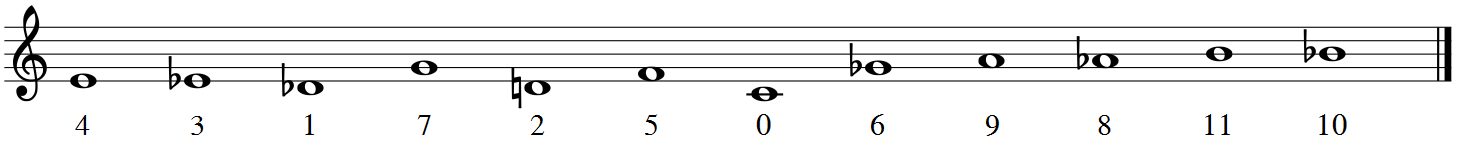
\includegraphics[width=\textwidth]{4.png}
	\bigskip\bigskip
	$$\text{IT}^6=\left(\begin{matrix}0&1&2&3&4&5&6&7&8&9&10&11\\10&9&7&1&8&11&6&0&3&2&5&4\\\end{matrix}\right)$$
	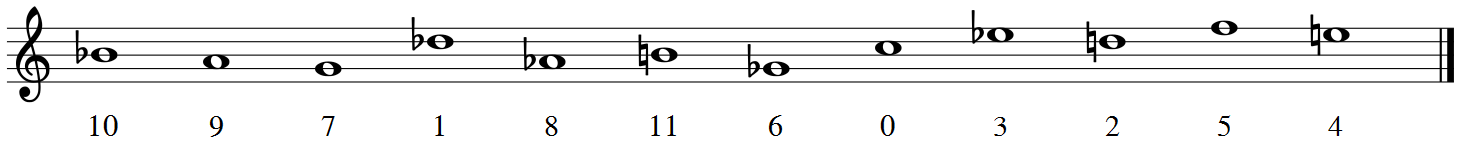
\includegraphics[width=\textwidth]{6.png}
	\newpage
	$$\text{RT}^0=\left(\begin{matrix}0&1&2&3&4&5&6&7&8&9&10&11\\10&9&0&11&2&8&3&6&1&7&5&4\\\end{matrix}\right)$$
	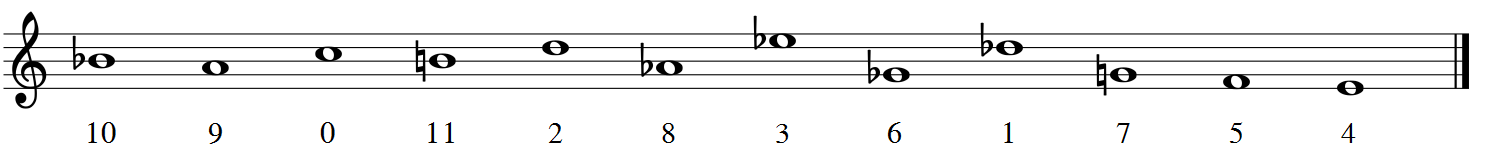
\includegraphics[width=\textwidth]{3.png}
	\bigskip\bigskip
	$$\text{RT}^6=\left(\begin{matrix}0&1&2&3&4&5&6&7&8&9&10&11\\4&3&6&5&8&2&9&0&7&1&11&10\\\end{matrix}\right)$$
	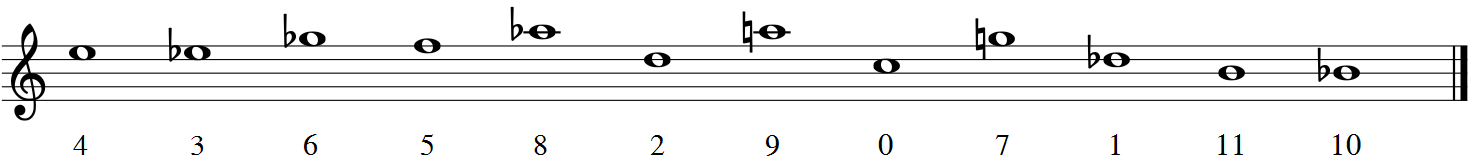
\includegraphics[width=\textwidth]{7.png}
	\bigskip\bigskip
	$$\text{IRT}^0=\left(\begin{matrix}0&1&2&3&4&5&6&7&8&9&10&11\\10&11&8&9&6&0&5&2&7&1&3&4\\\end{matrix}\right)$$
	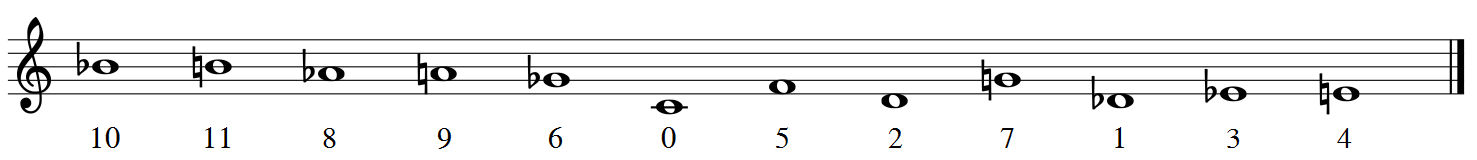
\includegraphics[width=\textwidth]{5.png}
	\bigskip\bigskip
	$$\text{IRT}^6=\left(\begin{matrix}0&1&2&3&4&5&6&7&8&9&10&11\\4&5&2&3&0&6&11&8&1&7&9&10\\\end{matrix}\right)$$
	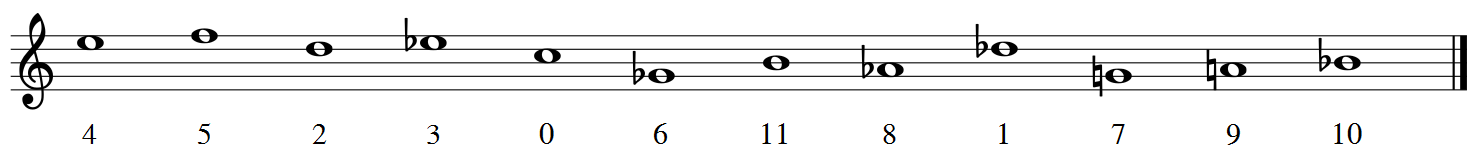
\includegraphics[width=\textwidth]{8.png}
		
		Estas series tienen muchos elementos en com�n: todas comienzan o acaban por mi$\natural$ o por si$\flat$, lo que permite enlazar unas series con otras por medio del un�sono o del tritono; se mantienen los intervalos de tritono en sus lugares originales o retr�grados, y coinciden en las dos primeras y las dos �ltimas notas dos a dos.
		
		Se han realizado estudios -- como el de Martha Hyde \cite{hyde} -- en los que se limitan las series utilizadas en la Suite a cuatro: $T^0$, $T^6$, $I$ e $IT^6$, pero ya que el objetivo de este texto no es analizar la obra entera se dejar� esta cuesti�n para an�lisis posteriores.
		
	\subsection{Descripci�n de la Suite op. 25}
		Schoenberg realiza en la serie $\sigma$ una partici�n triple; es decir, la serie se divide en tres tetracordios, y cada uno de ellos contiene un intervalo de tritono. El �ltimo tetracordio, si se retrograda, consta de las notas 10--9--0--11, que en notaci�n germ�nica es la secuencia BACH. Esto puede ser un homenaje al compositor Johann Sebastian Bach (1685\textemdash1750), ya que Schoenberg admiraba a los grandes compositores anteriores a �l por las estructuras formales de sus obras. Para m�s informaci�n, v�ase~\cite{xiao}.
		
		Otro posible homenaje a Bach y sus contempor�neos barrocos es precisamente la forma de la obra: es una Suite, g�nero cultivado durante los siglos XVII y XVIII que se compone de una variedad de danzas. La Suite de Schoenberg est� formada por seis danzas: un Preludio, una Gavota, una Musette, un Intermezzo \textemdash que no tiene influencia barroca sino m�s bien de Brahms, otro modelo para Schoenberg\textemdash, un Minueto con Tr�o y una Giga. Adem�s, el estilo, la textura \textemdash contrapunt�stica, t�picamente barroca\textemdash~ y la estructura de cada danza se corresponden con los estilos, texturas y estructuras de las danzas hom�nimas del periodo bachiano.
        
        Por ser �sta su primera obra totalmente dodecaf�nica, Schoenberg la utiliz� como una muestra al mundo de las posibilidades de su nuevo m�todo compositivo. Fue tambi�n por lo que tom� un formato tan variado como una Suite: as� pod�a en una misma obra componer con estilos tan distintos como los de las distintas danzas.
        
        Al componer la obra, Schoenberg trata cada tetracordio como una subunidad individual. Los superpone contra otras series del espectro tambi�n divididas, o utiliza sus notas como un solo acorde cuatr�ada. Estas divisiones no s�lo sirven para hacer la serie m�s reconocible o a�adir cohesi�n a la obra, sino que adem�s facilitan el desarrollo de la serie espec�ficamente en el estilo de cada danza.
		
	\subsection{An�lisis de la Musette}
	\label{musette}
		En el tercer movimiento de la Suite, la Musette, Schoenberg recrea la danza barroca que toma su nombre del instrumento hom�nimo: la \emph{cornamusa}, de la familia de la gaita. La m�sica compuesta para estos instrumentos suele consistir en una melod�a acompa�ada por una nota pedal, que se traduce aqu� en la presencia de un bord�n sobre el sol$\natural$ (nota 7). Esta nota se extrae de cada una de las series utilizadas y se forma con ella un ostinato r�tmico en la mano izquierda del piano. Con el resto de sonidos de cada serie, Schoenberg vuelve a emular el estilo de la danza barroca y articula un discurso polif�nico a dos voces con ritmos esencialmente cortos.
		
		A partir de la doble barra del comp�s 9, el re$\flat$ (nota 1) acompa�a a sol$\natural$ y ambos crean un doble bord�n en la mano izquierda. La elecci�n de esas dos notas est� estrechamente relacionada con la tradicional relaci�n de quinta justa formada por sol$\natural$ y re$\natural$ en la m�sica tonal. Schoenberg sustituye las quintas justas tonales por los tritonos dodecaf�nicos, subrayando a�n m�s su <<emancipaci�n de la disonancia>>.
		
		Adem�s de las similitudes texturales, r�tmicas y arm�nicas, la Musette de Schoenberg comparte estructura formal con las danzas barrocas. Y esta semejanza es quiz�s la m�s notable, ya que fue la b�squeda de estructura formal lo que inspir� a Schoenberg a desarrollar su m�todo compositivo. La Musette barroca, como todos los movimientos de danza, presenta una estructura binaria con simetr�a tonal: empieza y acaba por la misma tonalidad, mientras que el centro es zona de desarrollo. Schoenberg despoja de funcionalidad tonal a esa simetr�a, madre de la forma sonata, y la aplica a su composici�n dodecaf�nica.
		
		En este movimiento se pueden diferenciar a simple vista tres secciones, divididas en los compases 9 y 20, debido a cambios de textura, figuraci�n y tempo. En la segunda secci�n se le a�ade melod�a a la mano izquierda del piano, dejando m�s camuflado el bord�n que en la primera secci�n, adem�s de que �ste se vuelve doble, mientras que vuelve a aparecer claramente en la tercera secci�n. Tambi�n en la segunda secci�n aparece una nueva figuraci�n, que es la semicorchea; y, por �ltimo, en los dos compases de divisi�n aparecen dos \emph{a tempo}, que marcan el final de las dos primeras secciones tras dos zonas de variabilidad r�tmica.
		
		Para que esta estructura tr�ptica sea una forma binaria, la primera y la �ltima parte deben mantener un parecido, que se observa a trav�s del an�lisis de las series utilizadas en el movimiento. Estas series son $T^0$, $T^6$, $I$ e $IT^6$.
		
		En la Musette, Schoenberg hace un uso casi absoluto de la tripartici�n serial, hasta el punto de individualizar los tetracordios por separado y concederles privilegios seriales, como la retrogradaci�n. Por ejemplo, en el comp�s 7, en la voz inferior de la mano derecha aparece el tetracordio 4--5--2--3, que es o bien el primer tetracordio de $RIT^6$ o la retrogradaci�n del tercer tetracordio de $IT^6$, mientras que los otros dos tetracordios de $IT^6$, 10--9--7\footnote{La nota 7 aparece como bord�n y no en la misma voz que el resto del tetracordio, por lo que su posici�n es tambi�n excepcional.}--1 en la voz superior y 8--11--6--0 en la mano izquierda, aparecen en el orden correcto. Entonces no se puede analizar el comp�s como $RIT^6$, sino indicar que hay una alteraci�n puntual de $IT^6$.
		
		Por tanto, es muy complicado analizar esta obra en su totalidad, ya que la flexibilidad en la ordenaci�n de los tetracordios puede generar situaciones muy ambiguas. Debido a estas fragmentaciones y a las variadas combinaciones de tetracordios originales y retr�grados, se escucha un �rea de desarrollo hacia la secci�n media del movimiento. En cambio, las series al principio y al final de la pieza se presentan casi �ntegramente, como una exposici�n y reexposici�n. He aqu� un v�nculo con la simetr�a de las formas binarias tonales.
		
		Es m�s, incluso el orden de las series utilizadas en la primera y en la �ltima secci�n coinciden, exceptuando dos repeticiones consecutivas y las series $T^0$ finales, que act�an como una cadencia serial:
		
		\[\begin{array}{*{12}c}
			\mathbf{c}.\mathbf{1}&T^0&IT^6&T^6&I&T^0&I&T^6&
				\begin{matrix}IT^6&IT^6\\
				\end{matrix}
			&&&\mathbf{c}.\mathbf{9}\\
			\mathbf{c}.\mathbf{22}&T^0&IT^6&T^6&I&T^0&
				\begin{matrix}
				I&I\\
				\end{matrix}
			&T^6&IT^6&T^0&T^0&\mathbf{c}.\mathbf{31}\\\end{array}\]
		
		A continuaci�n se encuentra el an�lisis serial completo de la Musette:

\newpage
\begin{figure}[!h]
\begin{center}
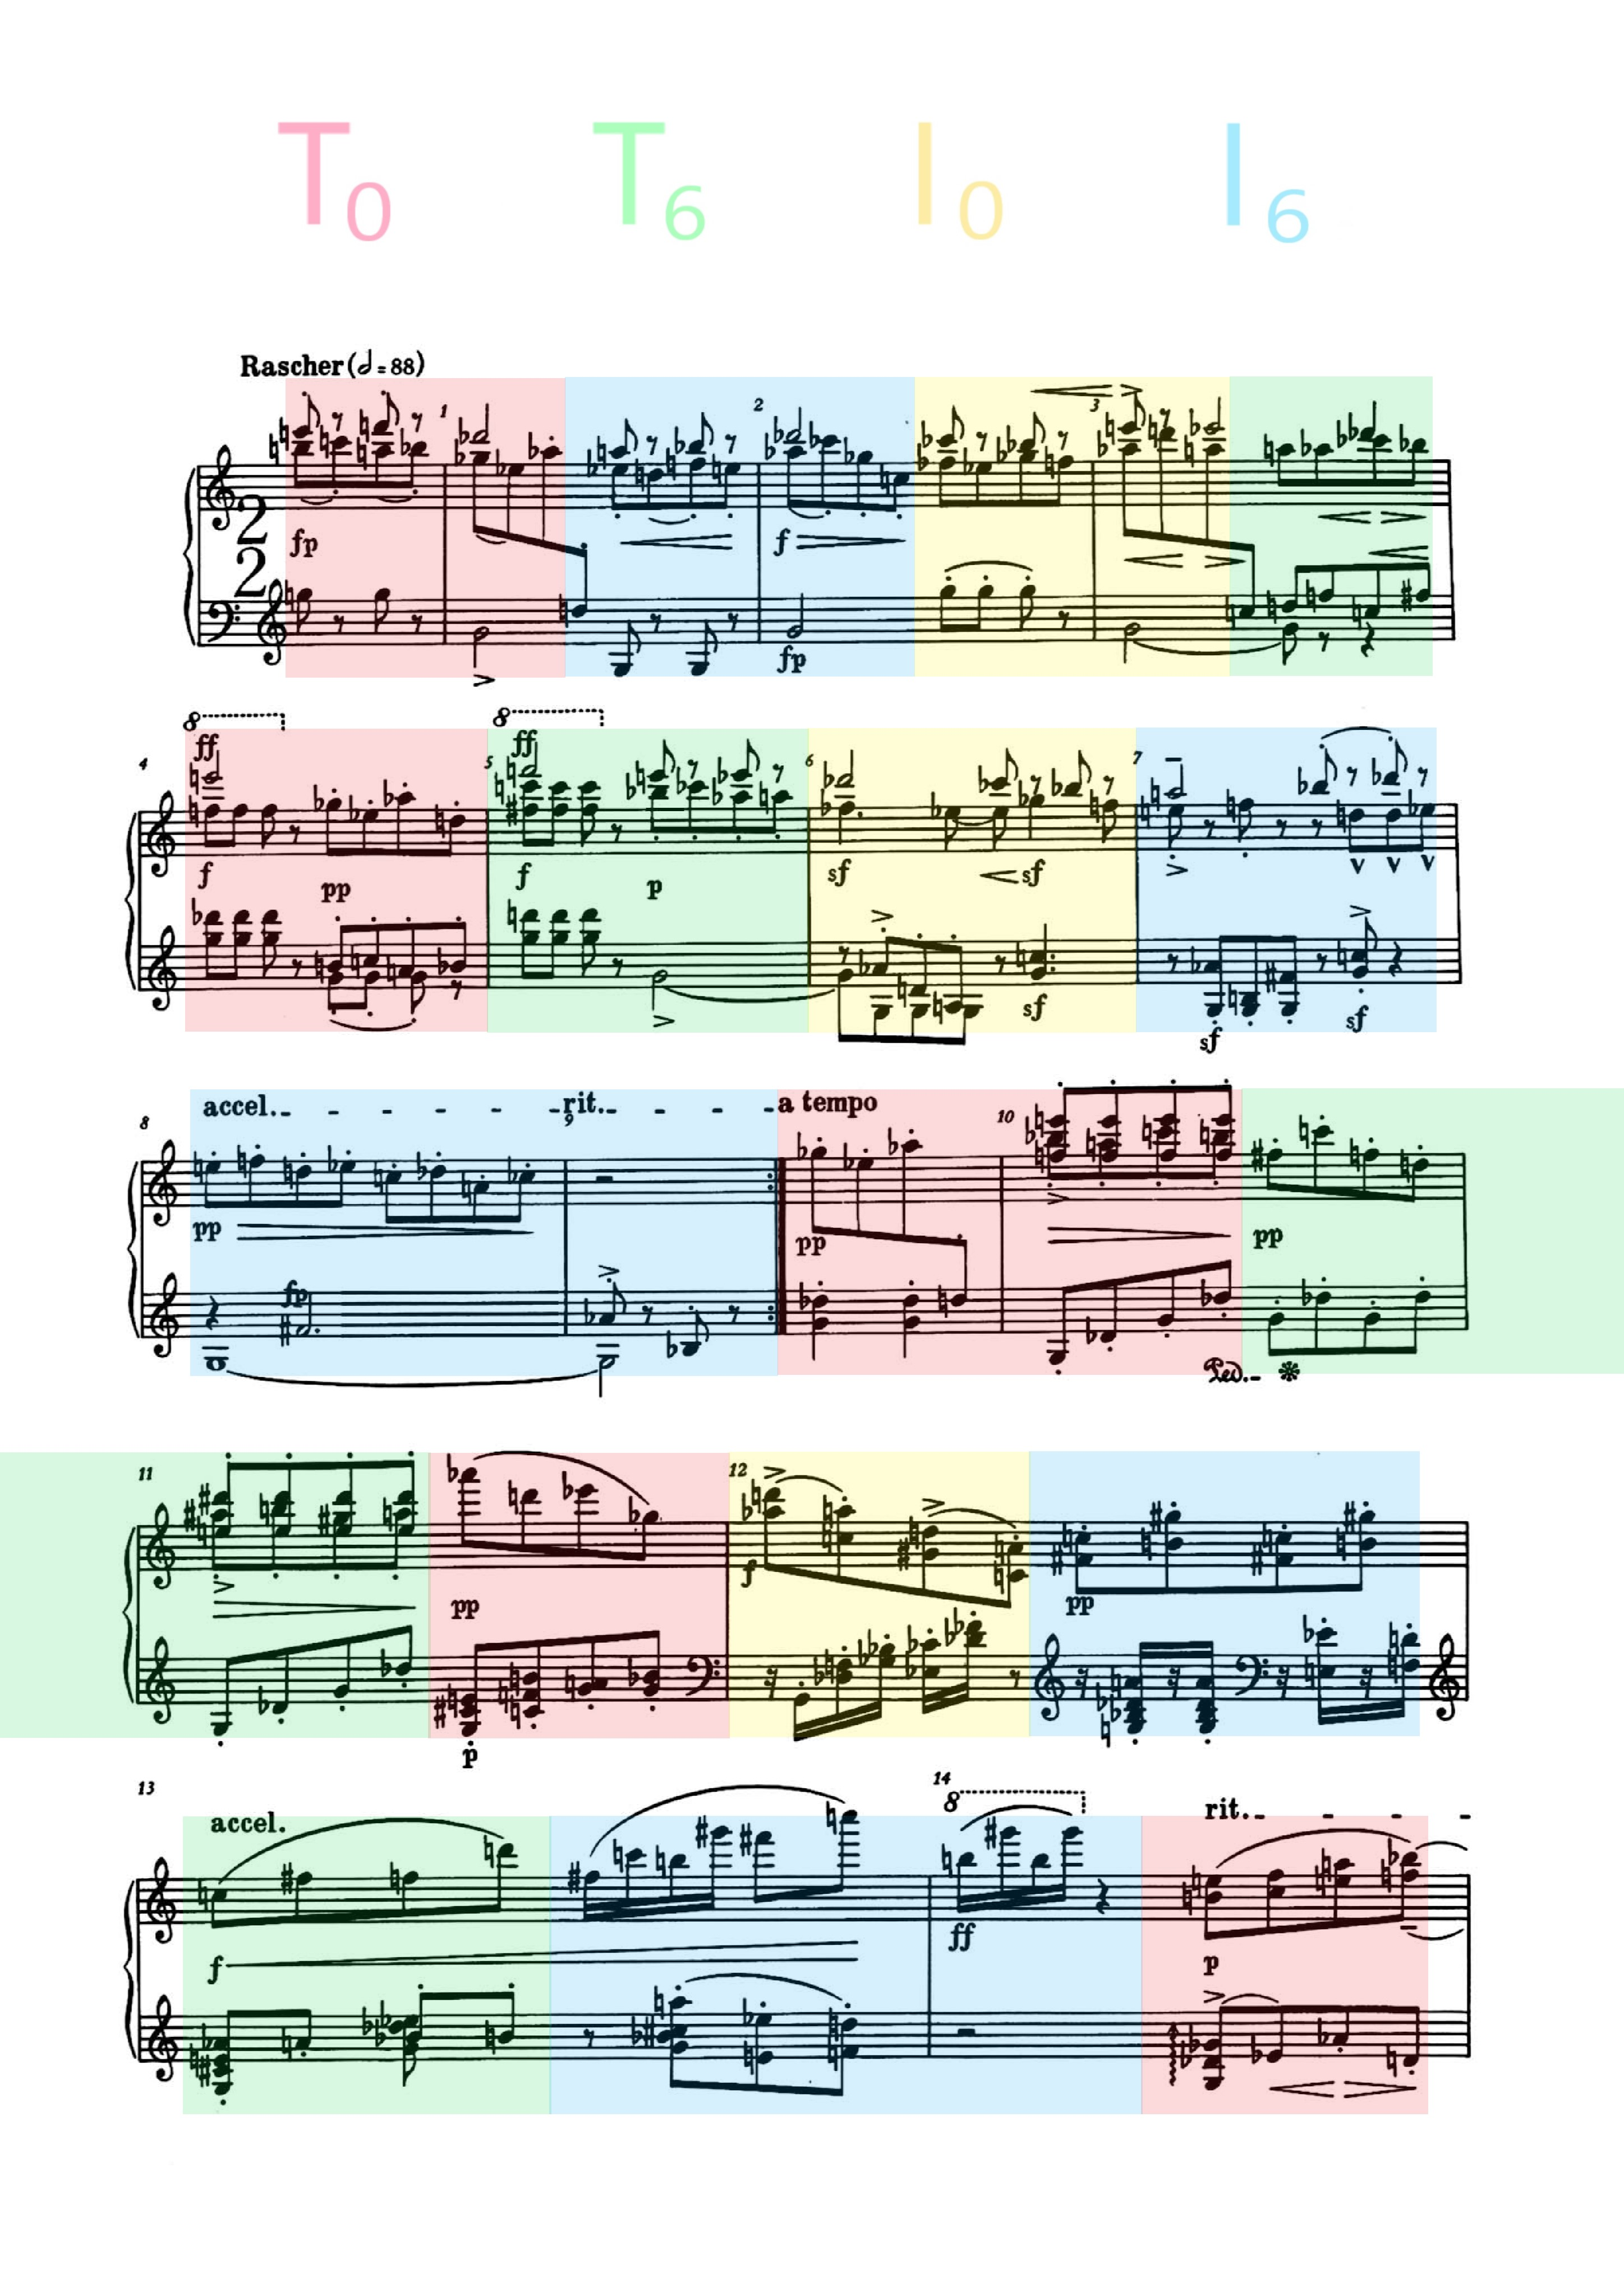
\includegraphics[width=14.5cm]{9.jpg}\\
\caption{An�lisis de la Musette (I)}
\end{center}
\end{figure}
$\,$


\newpage
\begin{figure}[!ht]
\begin{center}
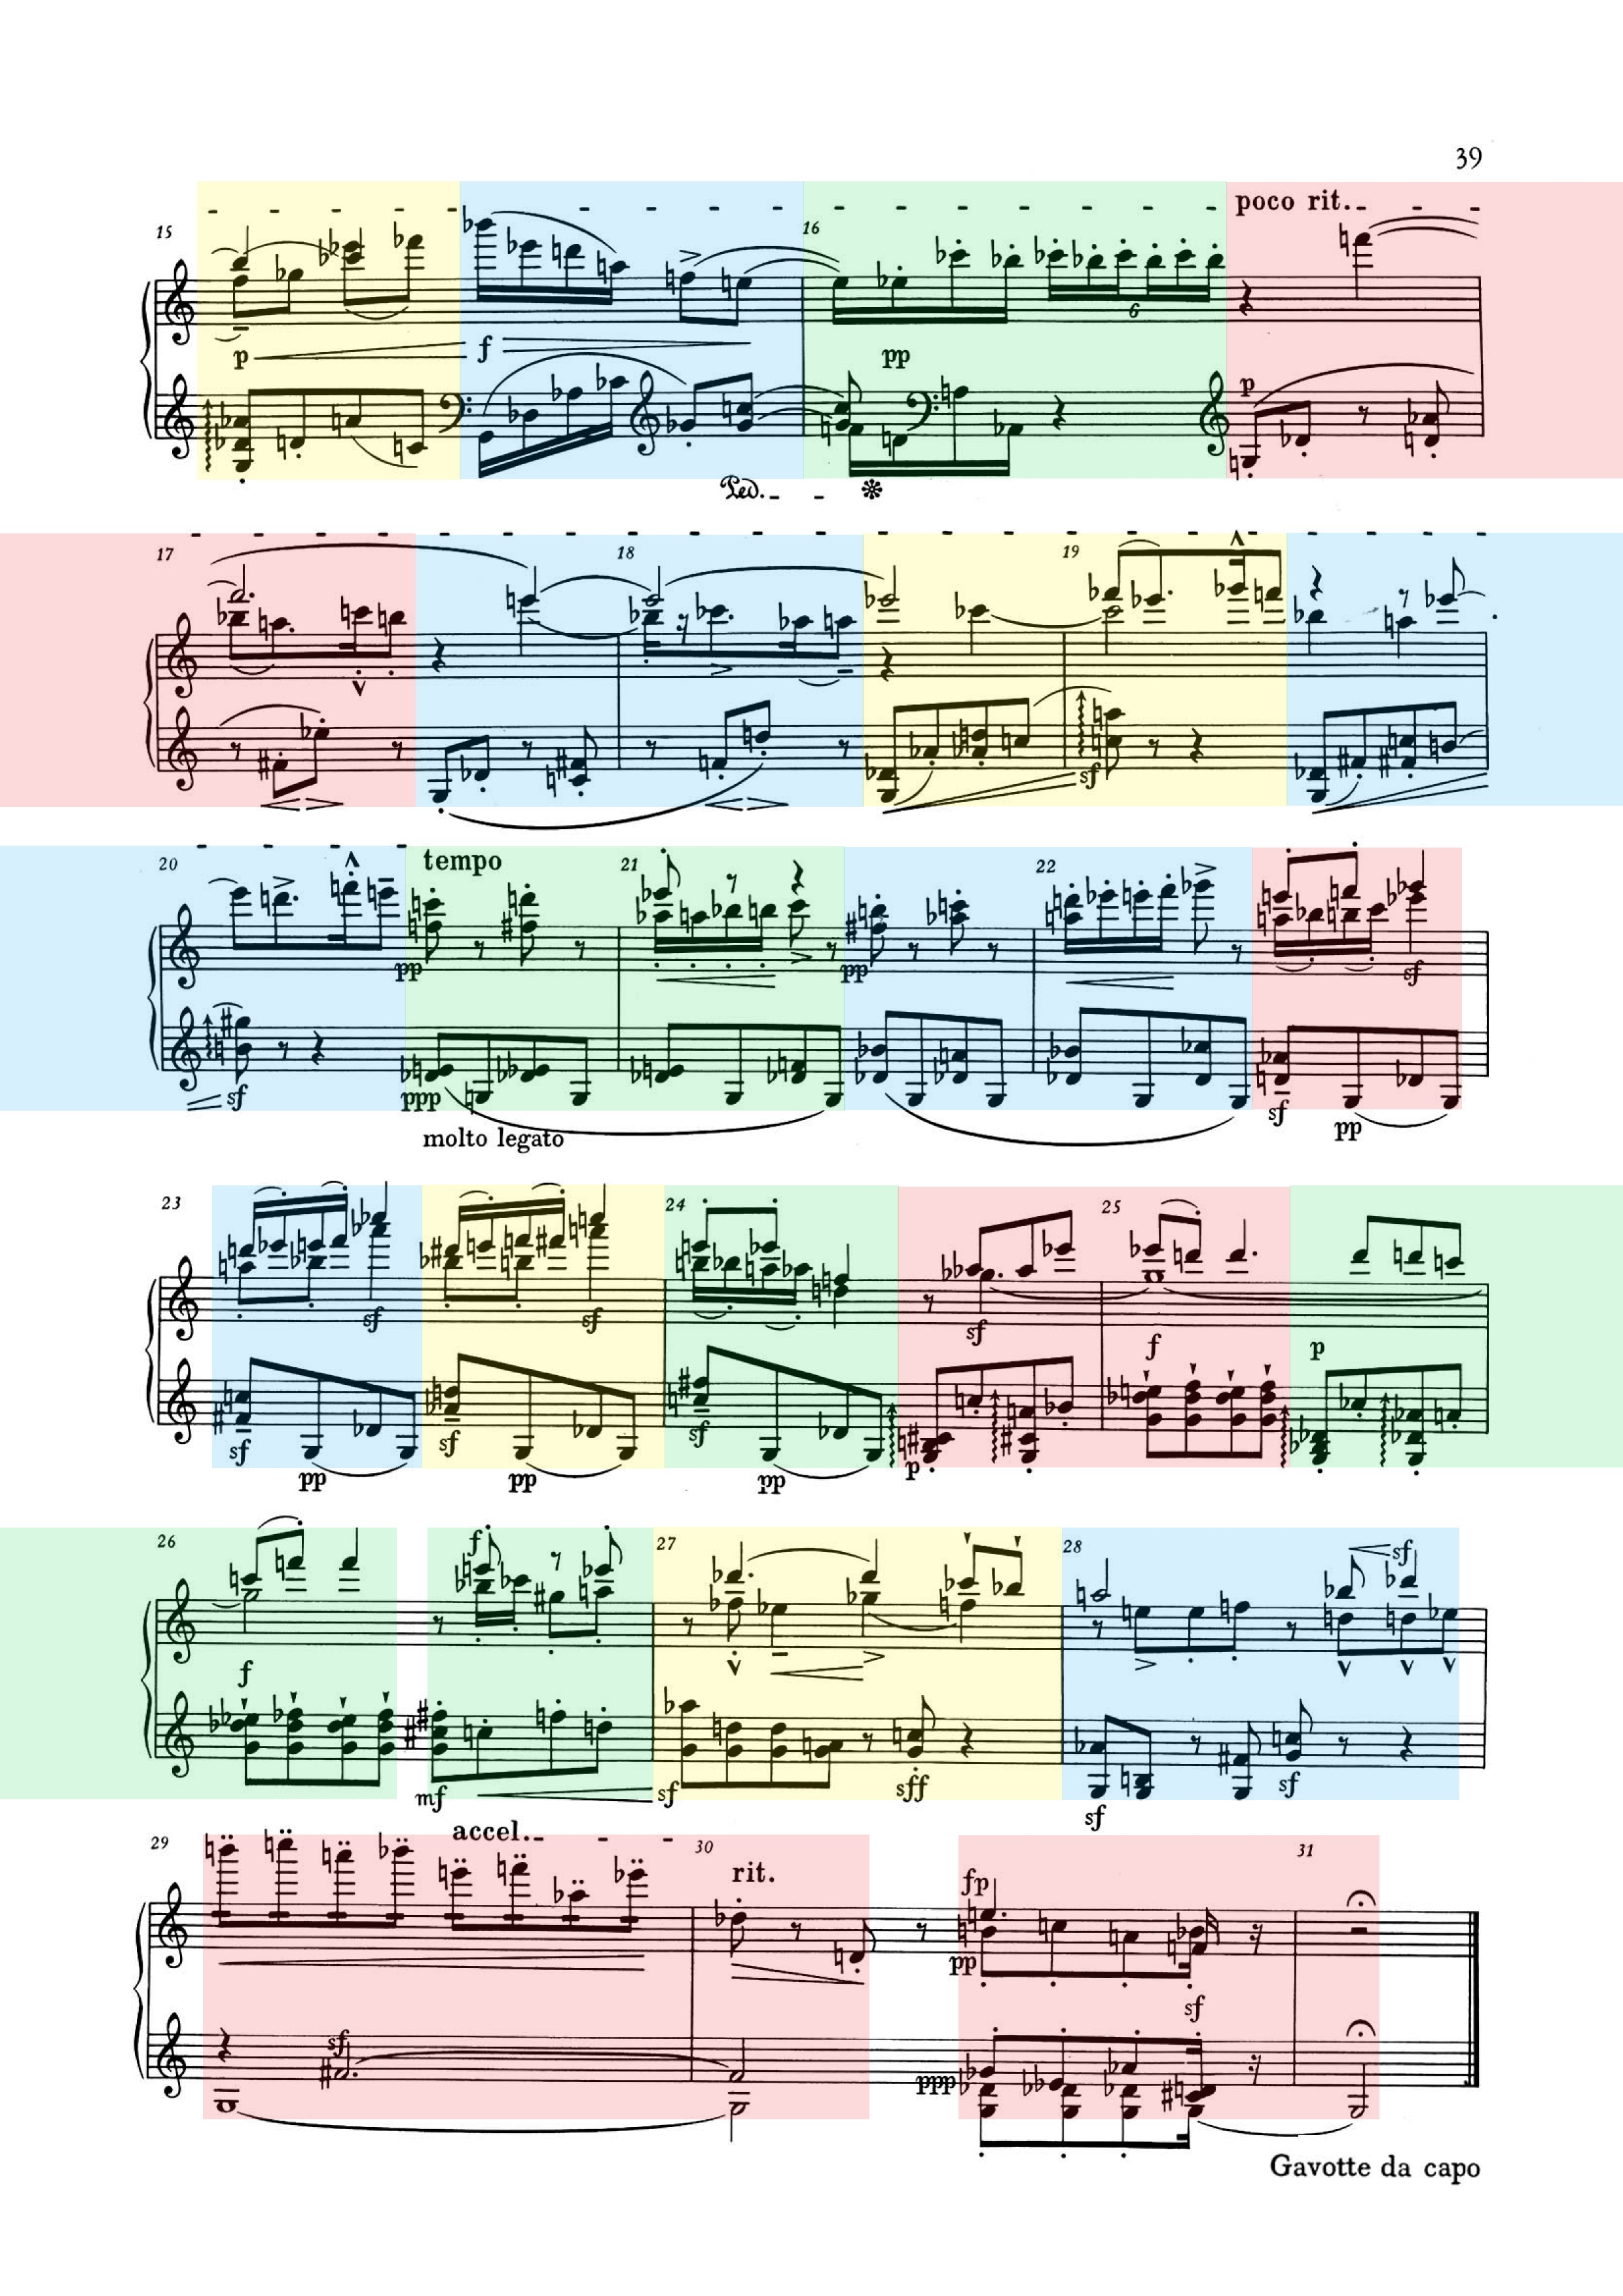
\includegraphics[width=14.5cm]{10.jpg}\\
\caption{An�lisis de la Musette (II)}
\end{center}
\end{figure}		
%
	\chapter{INTRODUCCIÓN MATEMÁTICA}
	\section{Conjuntos y grupos}
		Un \emph{conjunto} es una colección de objetos bien definidos y distintos entre sí que se llaman \emph{elementos}. 
	
		Para definir un conjunto se puede o bien listar los objetos uno a uno, o bien describirlos por medio de un predicado: una o varias propiedades que caracterizan a todos los elementos de dicho conjunto.

		Por ejemplo, el conjunto K$_\text{i}$, formado por las doce notas de la escala cromática de una misma octava i, está bien definido porque podemos hacer una lista con ellas: por ejemplo, $\text{K}_\text{4} = $
		
		\full{$\{\text{Do}_\text{4}, \text{Do\#}_\text{4}, \text{Re}_\text{4}, \text{Re\#}_\text{4}, \text{Mi}_\text{4}, \text{Fa}_\text{4}, \text{Fa\#}_\text{4}, \text{Sol}_\text{4}, \text{Sol\#}_\text{4}, \text{La}_\text{4}, \text{La\#}_\text{4}, \text{Si}_\text{4}\}$}
		
		Por un lado, aun llamando a las notas de distinta manera, el conjunto, conceptualmente, es el mismo. Además, el hecho de listar algún elemento más de una vez no afecta a su definición. Como $\text{Do\#}_\text{4} = \text{Re}\flat_\text{4}$,\footnote{En este texto se trabajará siempre con temperamento igual por convenio.}  $\text{K}_\text{4}$ también puede ser listado así:
		
		\full{$\{\text{Do}_\text{4}, \text{Do\#}_\text{4}, \text{Re}\flat_\text{4}, \text{Re}_\text{4}, \text{Re\#}_\text{4}, \text{Mi}_\text{4}, \text{Fa}_\text{4}, \text{Fa\#}_\text{4}, \text{Sol}_\text{4}, \text{Sol\#}_\text{4}, \text{La}_\text{4}, \text{La\#}_\text{4}, \text{Si}_\text{4}\}$}
	
		En cambio, el conjunto D, formado por las duraciones rítmicas elementales -- sin ligaduras ni puntillos --, es infinito, por lo que no se puede listar de forma completa. Sin embargo, se puede expresar por medio de un predicado:
		
		\full{$\text{D} =\{2^n:n\in\mathbb{Z},\ n\le 2\} = \{4,\ 2,\ 1,\ \frac{1}{2},\ \frac{1}{4},\ \frac{1}{8},\ \ldots\} = \{\fullnote,\ \halfnote,\ \quarternote,\ \eighthnote,\ \ldots\}$}
		
		La notación $n\in\mathbb{Z}$ significa que $n$ pertenece a los números enteros. En este caso se han representado las duraciones mediante su ratio con la duración de la negra $\quarternote$.
	
		Los elementos de un conjunto pueden combinarse mediante \emph{operaciones} -- como la suma o la multiplicación en el caso de los números -- para dar otros objetos matemáticos. 
		
		Se dice que un conjunto G no vacío y una operación binaria ($\ast$) forman la estructura de un \emph{grupo} (G, $\ast$) cuando cumplen:
	
		\begin{enumerate}
			\item{Su operación es interna: Si $a,b\in$ G, entonces $a\ast b\in$ G.}		
			\item{Su operación es asociativa: Si $a,b,c\in$ G, $(a\ast b)\ast c=a\ast(b\ast c)$. }
			\item{Existe un elemento $e$ en G, llamado elemento neutro o identidad, tal que para todo $x\in$ G se cumple que $e\ast x = x\ast e = x$. Se puede probar que el neutro es único para cada grupo. A veces se incluye dentro de la definición del grupo: (G, $\ast$, $e$).}
			\item{Cada $x\in$ G tiene asociado otro elemento $x^{-1}\in$ G, llamado elemento inverso, tal que $x \ast x^{-1} = x^{-1}  \ast x = e$. Se puede probar que el inverso de cada elemento es único.}		
		\end{enumerate}
	
	($\mathbb{Z},+,0$) y ($\mathbb{Q},+,0$) son grupos, pero ($\mathbb{N},+,0$) no porque no existe el \textit{inverso} de 2 con la suma: $-2\notin\mathbb{N}$. ($\mathbb{R},*,1$) y ($\mathbb{Q},*,1$) son grupos, pero ($\mathbb{Z},*,1$) no porque no existe el \textit{inverso} de 2 con la multiplicación: $\frac12\notin\mathbb{Z}$.
	
	\section{Funciones y permutaciones}
		Una \emph{función} es una regla que asocia a cada elemento de un primer conjunto, llamado \emph{dominio}, un único elemento de un segundo conjunto. Si la función se llama $f$, el dominio A y el segundo conjunto B, se denota $f:\text{A}\to \text{B}$. El elemento asociado a un $x$ mediante $f$ se denota $f(x)$.
		
		Todos los $x\in$ A tienen que estar asociados a un $f(x)\in$ B, pero no todos los elementos de B tienen un elemento de A asociado. Los elementos de B que sí lo cumplen, es decir, los que se pueden escribir como $f(x)$ para algún $x$, forman el conjunto \emph{imagen} de la función: $im(f)=\{\ y\in \text{B}:\ \exists\ x \in \text{A},\ f(x)=y\ \}$
		
		Cuando varias funciones se aplican una detrás de la otra decimos que realizamos la operación de \textit{composición de funciones}. Se representa con el símbolo $\circ$. La imagen de la primera función será el dominio de la segunda, y así sucesivamente. Por ejemplo, aplicar una función $f(x)$ y después aplicar una función $g(x)$ se denota $g(f(x))=(g\circ f)(x)$.
		
		Una \emph{permutación} $\sigma$(X) es una función sobre un conjunto X que asocia sus elementos a los elementos del mismo conjunto X de manera unívoca. Es decir, asocia cada elemento a uno, y solo uno, de los elementos de su mismo conjunto ($\sigma:\text{X}\to \text{X}$).

		El conjunto de todas las posibles permutaciones sobre un determinado conjunto X, junto con la operación de composición de funciones ($\circ$), forma un grupo denotado por S$_\text{x}$. Para probarlo, se debe comprobar que cumple todas las propiedades de los grupos.

		\begin{enumerate}
			\item{Permutar dos veces es también una permutación.}
			\item{La composición de funciones es asociativa.}
			\item{La permutación que asigna un elemento a sí mismo es la función identidad.}
			\item{Como las permutaciones son biyectivas, cada una tiene una inversa que es también una permutación.}		
		\end{enumerate}

		Cuando X es el conjunto de números naturales desde 1 hasta $n$, el grupo S$_\text{x}$ se representa como S$_n$ y se le denomina el grupo simétrico de orden $n$. El número de elementos en S$_n$, es decir, de posibles permutaciones de $n$ números, es $n!$. 
		
		En los ejemplos musicales de este texto, los conjuntos estarán numerados desde 0 hasta $n-1$, siendo $n$ el número de elementos a permutar, en vez de desde 1 hasta $n$. Seguirán siendo grupos simétricos de orden $n$, pero con una numeración distinta.
		
		La notación utilizada para representar una permutación $\sigma$ perteneciente a S$_n$ con la numeración desde 0 y con $\sigma(m)$ siendo el elemento asociado a $m$ mediante $\sigma$, es:
		\[\sigma=\left(\begin{matrix}0&1&2&&n-3&n-2&n-1\\\sigma\left(0\right)&\sigma\left(1\right)&\sigma\left(2\right)&\cdots&\sigma\left(n-3\right)&\sigma\left(n-2\right)&\sigma\left(n-1\right)\\\end{matrix}\right)\]
		
	\section{Aritmética modular básica}
		Fijado un $n\in\mathbb{N}$, se dice que $a$ y $b$ son \textit{congruentes} (o equivalentes) módulo $n$ si tienen el mismo resto al dividirlos entre $n$; es decir, que todos los números con el mismo resto se agrupan y se toman como equivalentes. Se expresa como $a\equiv b$ (mod. $n$).
	
		De esta forma se pueden operar entre sí los números del 0 al $n-1$, ya que se conservan las operaciones de los números enteros, y si un resultado es $\geq n$ se puede seguir dividiendo entre $n$ para que cumpla $0\leq r<n$.
		
		Se conserva la suma (y la resta), ya que si $a=nq_a+r_a$ y $b=nq_b+r_b$, entonces $a+b=(nq_a+r_a)+(nq_b+r_b)=n(q_a+q_b)+(r_a+r_b)$, así que el resto de $a+b$ es igual al de $r_a+r_b$.
		
		La \textit{aritmética modular} también se llama aritmética del reloj, porque funciona de la misma manera que las horas en un reloj. Como el 3 tiene el mismo resto entre 12 que el 15, las 15h son las 3h: $3\equiv15$ (mod. $12$). O, por ejemplo, 2 horas después de las 11 dan las 13, es decir, la 1: $2+11=13\equiv1$ (mod. $12$). 
		
		También se conserva la multiplicación: si $a=nq_a+r_a$ y $b=nq_b+r_b$, entonces $ab=(nq_a+r_a)(nq_b+r_b)=n^2q_aq_b+nq_ar_b+nq_br_a+r_ar_b=n(nq_aq_b+q_ar_b+q_br_a)+r_ar_b$, así que el resto de $ab$ es igual al de $r_ar_b$.
		
		En música, la aritmética modular se puede encontrar en las escalas: todas las notas Do se toman como equivalentes, por ejemplo, y al sumarle 12 semitonos (una octava) se vuelve a obtener un Do. Si se asocian los números del 0 al 11 a las notas cromáticas del Do al Si, entonces $0+12=12\equiv0$ (mod. $12$).%
	
		\begin{thebibliography}{00}
		\addcontentsline{toc}{chapter}{Bibliografía}
			
%			\item Introducción:
			
			\bibitem{wright}
			{\sc Wright, David.} 
			\textit{Mathematics and Music},
			American Mathematical Society 
			(2009).
			
%			\item Historia:
			
%			\bibitem{kinney}
%			{\sc Kinney, James P.} 
%			\textit{Twelve-tone Serialism: Exploring the Works of Anton Webern},
%			Undergraduate Honors Theses.
%			Paper 1
%			(2015)
%			
%			\bibitem{diaz}
%			{\sc Díaz de la Fuente, Alicia.} 
%			\textit{Estructura y significado en la música serial y aleatoria},
%			Universidad Nacional de Educación a Distancia.
%			Tesis Doctoral en Filosofía
%			(2005)
%			
%			\bibitem{delgado}
%			{\sc Prof. Fernando Delgado García.} 
%			Clases y material de Historia de la Música, 5$^{\circ}$ y 6$^{\circ}$ de Enseñanzas Profesionales del Conservatorio Profesional de Música Arturo Soria, cursos 2014-15 y 2015-16.
			
%			NADA
%			\bibitem{dominguez}
%			{\sc Domínguez Romero, Manuel.} 
%			\textit{Las Matemáticas en el Serialismo Musical},
%			Sigma n.24 
%			(2004).

%			\item Suite:
					
%			\bibitem{xiao}
%			{\sc Xiao, June.} 
%			\textit{Bach’s Influences in the Piano Music of Four 20th Century Composers},
%			Indiana University Jacobs School of Music.
%			Doctoral Theses in Music
%			(2014)
%			
%			\bibitem{clercq}
%			{\sc Clercq, Trevor de.} 
%			\textit{A Window into Tonality via the Structure of Schoenberg's ``Musette'' from the Piano Suite, op. 25},
%			Theory/Analysis of 20th-Century Music.
%			Prof. David Headlam
%			(2006)
%			
%			\bibitem{hyde}
%			{\sc Hyde, Martha.} Chapter 4: “Dodecaphonism: Schoenberg”,
%			\textit{Models of Musical Analysis: Early Twentieth-century Music},
%			Ed. Mark Everist and Jonathan Dunsby.
%			Oxford: Blackwell
%			(1993)
%			
%			\bibitem{ilomaki}
%			{\sc Ilom\"aki, Tuukka.}
%			\textit{On the Similarity of Twelve-Tone Rows},
%			Sibelius Academy
%			(2008).
			
%			\item Acciones:
			
%			\bibitem{armstrong}
%			{\sc Armstrong, M. A.} Chapter 6: “Permutations”, Chapter 17: “Actions, Orbits, and Stabilizers”, Chapter 18: “Counting Orbits”,
%			\textit{Groups and Symmetry},
%			New York: Springer-Verlag
%			(1988)
			
%			\item Espectros:
			
			\bibitem{polygons}
			{\sc Golomb, S. W., Welch, L. R.}
			\textit{On the enumeration of polygons},
			The American Mathematical Monthly, Vol. 67, 349-353
			(1960).
			
			\bibitem{reiner}
			{\sc Reiner, David L.}
			\textit{Enumeration in Music Theory},
			The American Mathematical Monthly, Vol. 92, No. 1
			(1985).
			
%			\item Filosofía:
			
%			\bibitem{basomba}
%			{\sc Basomba García, Daniel.} 
%			\textit{El último Bach y el dodecafonismo como ideal musical: una lectura estética y sociológica},
%			Universidad Carlos III de Madrid.
%			Tesis Doctoral en Ciencia Política y Sociología
%			(2013)
			
%			NADA
%			\bibitem{bhalerao}
%			{\sc Bhalerao, Rasika.} 
%			\textit{The Twelve-Tone Method of Composition},
%			Math 336.
%			Prof. Jim Morrow
%			(2015)
			
%			NADA
%			\bibitem{morris}
%			{\sc Morris, Robert.}
%			\textit{Mathematics and the Twelve-Tone System: Past, Present, and Future},
%			Perspectives of New Music 45.2 
%			(2007)
			
%			NADA
%			\bibitem{cook}
%			{\sc Cook, Nicholas.} Chapter 9: “Analyzing Serial Music”,
%			\textit{A Guide to Musical Analysis},
%			New York: G. Braziller
%			(1987)
			
%			NADA
%			\bibitem{roberts}
%			{\sc Roberts, Gareth E.}
%			\textit{Composing with Numbers: Arnold Schoenberg and His Twelve-Tone Method},
%			Math/Music: Aesthetic Links
%			(2012).
			
%			NADA
%			\bibitem{hunter}
%			{\sc Hunter, David J.; von Hippela, Paul T.}
%			\textit{How Rare Is Symmetry in Musical 12-Tone Rows?},
%			The American Mathematical Monthly, Vol. 110, No. 2
%			(2003).
			
%			NADA
%			\bibitem{rowdata}
%			{\sc London, J., von Hippel, P., Huron, D., Cartano, J., Kingery, K., Olsen, B., Santelli, T.}
%			\textit{Row forms in the serial works of Schoenberg, Berg, and Webern}
%			[Computer database.] Stanford, CA: Center for Computer Assisted Research in the Humanities (www.ccarh.org/publications/data/humdrum/tonerow/) (2000/2001).
						
	\end{thebibliography}

\end{document}
